%! TEX option=--shell-escape
\documentclass[12pt,a4paper,openright,twoside]{report}

\usepackage[utf8]{inputenc}
\usepackage[spanish]{babel}
\usepackage{amsmath}
\usepackage{amsfonts}
\usepackage{amssymb}
\usepackage{graphicx}

\usepackage{lmodern,textcomp}
%Paquete para ajustar el tamaño de pagina, margenes, etc
\usepackage{geometry}
%geometría definida respecto a las sugerencias
  \geometry{
  	includehead,
  	includefoot,
  	a4paper,
  	left = 20mm,
  	top = 25mm,
  	total ={170mm,257mm},
  }
%El siguiente paquete provee las funciones necesarias para ajustar el encabezado
%y el pie de página
\usepackage{fancyhdr}
  \pagestyle{fancy}
  \fancyhf{} % resetea el encabezado y el pie
  \fancyhead[LE,LO]{\fontsize{9pt}{1pt}\it \leftmark}
  \fancyfoot[LE,RO]{\fontsize{12pt}{1pt}\thepage}


  \fancypagestyle{plain}{
  	\fancyfoot[RE,RO]{\fontsize{12pt}{1pt}\thepage}}

%usado para colocar la fecha en la carátula
\usepackage{datetime}

\setlength{\parskip}{\baselineskip}
%\renewcommand{\topfraction}{.85}
\renewcommand{\bottomfraction}{.7}
%\renewcommand{\textfraction}{.15}
%\renewcommand{\floatpagefraction}{.66}
%\renewcommand{\dbltopfraction}{.66}
%\renewcommand{\dblfloatpagefraction}{.66}

\usepackage{listings}
\usepackage{listingsutf8}
\lstset{inputencoding=utf8/latin1}
\lstset{tabsize=4}
\usepackage{caption}
\usepackage{subcaption}
\usepackage{enumerate}
\usepackage{lineno}
\usepackage{array}
\usepackage{booktabs}
\usepackage[titletoc]{appendix}
\usepackage{pdfpages}
%\usepackage[section]{placeins}

\usepackage[binary-units]{siunitx}
\usepackage{titling}
\usepackage{soul}
\usepackage{adjustbox}

%change captions name of table using babel
\renewcommand{\spanishtablename}{Tabla}

\usepackage{hyperref}
\hypersetup{
	colorlinks=false,
	linkcolor=black,
	filecolor=black,
	urlcolor=black,
	pdftitle={\@title},
	bookmarks=true,
	hidelinks
}

\usepackage{tikz}
\usetikzlibrary{arrows,backgrounds,decorations.pathreplacing,fit,positioning,petri,babel,shapes,circuits.logic.mux,circuits.logic.US,shapes.gates.logic,trees,patterns}

%\tikzstyle{style} = [definition]
\tikzstyle{interior}=[rectangle,rounded corners,draw=black,minimum size=3em, text width=20,fill=white]
\tikzstyle{exterior} = [rectangle,draw=black,minimum size=40]
\tikzstyle{mode text} = [midway,sloped,text width=200]
\tikzstyle{contenedor} = [rectangle,draw=black]
\tikzstyle{core}=[interior]
\tikzstyle{perif} = [interior,minimum height=20]
\tikzstyle{buf}=[core, text width=53, align=center]
\tikzstyle{obuf} = [buf, node distance=.7]
\tikzstyle{env} = [fill=black!20]
\tikzstyle{simple}=[rectangle, draw=black, minimum height=220, text width=65,align=center]
\tikzstyle{moore} = [rectangle,draw=black, minimum height= 30,text width=80,align=left]
\tikzstyle{mealy} = [rectangle,rounded corners=12, draw=black, text width = 80,align=left,minimum height=40]
\tikzstyle{ask} = [diamond,text width=50,draw=black,align=center,]
\tikzstyle{bloque}=[exterior,align=center,minimum size=60,text width=60]
\tikzstyle{hub}=[draw=black,anchor=west,circle]
\tikzstyle{dev}=[draw=black,anchor=west,rectangle,rounded corners,text width=60,align=center]
\tikzstyle{pid}=[draw=black,align=center,rectangle,rounded corners,minimum width=20,minimum height=75,pattern=north east lines,pattern color=black!35]
\tikzstyle{dir}=[draw,rectangle,rounded corners,minimum width=20,minimum height=75,align=center]
\tikzstyle{data}=[draw=black,align=center,rectangle,rounded corners,minimum width=80,minimum height=75,fill=black!05]
\tikzstyle{crc}=[draw=black,align=center,rectangle,rounded corners,minimum width=20,minimum height=75,pattern=dots,pattern color=black!25]
\tikzstyle{field}=[draw=black,rectangle,rounded corners, minimum height=30,align=center]
\tikzstyle{chart}=[circle,draw=black,text width=50,align=center]
\tikzstyle{lineaExt} = [->,line width=5pt, >=latex, shorten <= 1]
\tikzstyle{lineaInt} = [->,line width=3pt,white, shorten >= 4.8, >=latex, shorten <= 2]


\newcommand{\epg}[3]{
	Buffer {#1}\\
	[38.5pt]EP{#2}\\
	[38.5pt]{#3} Bytes}

\newcommand{\ep}[3]{
	Buffer {#1}\\
	[8pt]EP{#2}\\
	[8pt]{#3} Bytes}

\newcounter{wavecount}

\newcommand{\newwave}[1]{
	\path (0,\value{wavecount}) node[text width=70,anchor=east,align=right]{#1} node[coordinate](t_cur){};
	\draw (0,\value{wavecount}+.3) --++(.2,0);
	\draw (0,\value{wavecount}-.3) --++(.2,0);
	\path (t_cur) --++(.3,0)node[coordinate](t_cur){};
	\addtocounter{wavecount}{-1}}

\newcommand*{\bit}[2]{
	\draw (t_cur) -- ++(0.1,.6*#1-.3) -- ++(#2-.2,0) -- ++(+.1,.3-.6*#1)
	node[coordinate] (t_cur) {};}

\newcommand*{\bitvector}[2]{
	\draw[] (t_cur) -- ++( .1, .3) -- ++(#2-.2,0) -- ++(.1, -.3)
	-- ++(-.1,-.3) -- ++(.2-#2,0) -- cycle;
	\path (t_cur) -- node[align=center] {#1} ++(#2,0) node[coordinate] (t_cur) {};}

\newcommand*{\graybitvector}[2]{
	\draw[fill=black!15] (t_cur) -- ++( .1, .3) -- ++(#2-.2,0) -- ++(.1, -.3)
	-- ++(-.1,-.3) -- ++(.2-#2,0) -- cycle;
	\path (t_cur) -- node[align=center] {#1} ++(#2,0) node[coordinate] (t_cur) {};}

\DeclareSIUnit[number-unit-product = {}]
\byte{B}

\graphicspath{{./imgs/}}

\renewcommand{\chaptermark}[1]{%
    \markboth{\thechapter.\ #1}{}}

\lstset{literate=
	{á}{{\'a}}1	{é}{{\'e}}1	{í}{{\'i}}1	{ó}{{\'o}}1	{ú}{{\'u}}1	{α}{{$\alpha$}}1	{β}{{$\beta$}}1	{γ}{{$\gamma$}}1	{ñ}{{\~n}}1
}

\renewcommand{\appendixpagename}{Apéndice}
\renewcommand{\labelitemi}{$\bullet$}
\renewcommand{\labelitemii}{$-$}

% Las próximas líneas son archivos que conviene que estén por aquí

	%bridge.c
\newcommand{\bridge}{secciones/cuerpo/capitulo3/bridge.c}
\newcommand{\host}{USB Host}
\newcommand{\device}{Dispositivo USB}
\newcommand{\devices}{Dispositivos}
\newcommand{\endpoint}{Extremo}
\newcommand{\hub}{Distribuidor USB}
\newcommand{\function}{Función USB}
\newcommand{\functions}{Funciones USB}


\lstset{literate=
	{á}{{\'a}}1	{é}{{\'e}}1	{í}{{\'i}}1	{ó}{{\'o}}1	{ú}{{\'u}}1	{α}{{$\alpha$}}1	{β}{{$\beta$}}1	{γ}{{$\gamma$}}1	{ñ}{{\~n}}1
}
\title{Desarrollo e implementación de un puerto USB 2.0 de alta velocidad para
	FPGA a través de un puente específico}
\author{Edwin Barragán}

\begin{document}
%	\renewcommand{\tablename}{Tabla}
	\begin{titlepage}
  \begin{center}
    \begin{Large}
      \textbf{UNIVERSIDAD NACIONAL DE SAN JUAN\\
      \vspace*{0.05in}
      FACULTAD DE INGENIERIA\\
      \vspace*{0.05in}
      Departamento de Electrónica y Automática\\
      \vspace*{0.2in}
      \includegraphics[width=.3\textwidth]{logo_unsj.png}\\
      \vspace*{\fill}}
    \end{Large}
    \begin{Large}
      \textbf{Trabajo Final\\\MakeUppercase{\thetitle}} \\
      Informe\\
    \end{Large}
    \vspace*{\fill}
    \begin{large}
      \textbf{\theauthor}\\
      Autór\\
    \end{large}
    \vspace*{0.5in}
    \begin{large}
      \textbf{Ing.~Cristian~Sisterna \hspace*{\fill}
      Mgtr.~Ing.~Martín~Pérez \hspace*{\fill} Dr.~Marcelo~Segura \\}
      Asesores\\
    \end{large}
    \vspace{\fill}
    \rule{80mm}{0.1mm}\\
    \vspace{.1in}
    \the\year
  \end{center}

\end{titlepage}

	\null
	\chapter*{Agradecimientos}
A mi familia. Cimiento de lo que soy. Apoyo incondicional. Modelos de esfuerzo y dedicación. A Victorina y María Cristina. A Cristina y Francisco. A Ana María, Ricardo, Javier y Gabriela. A Bernardo, Valeria, Agustín, Joaquín y Sofía. Los quiero con el alma.

A Martín, por su guía y consejo. Por su marca constante, para lograr un buen resultado.

A Alfredo y Adriana, por su apoyo y comprensión. Aporte infinito a la concreción de este trabajo.

A Natalia, mi compañera, mi amor incondicional. Por el aguante y aliento permanente.

A cada uno de los profesores que con su enseñanza me formaron como profesional.

A mis compañeros, a los ocasionales, pero fundamentalmente a los de siempre. A los miembro del GERUNSJ, parte muy importante de mi formación.

A mis amigos, fundamentalmente a mi nueva familia de Bariloche, que hacen que la distancia sea más agradable y liviana.

A todos ellos, mi infinito agradecimiento.
	\tableofcontents
	\printglossary[type=\acronymtype,title={Lista de Acrónimos},nonumberlist]
	\chapter{Introducción}
	\section{Motivación}
		El presente informe busca dar a conocer al lector las tareas y actividades desarrolladas por el autor, a fin de dar cuenta sobre lo realizado en el marco del Trabajo Final de la carrera Ingeniería Electrónica, dictada en la Facultad de Ingeniería de la Universidad Nacional de San Juan.\\

El objetivo principal de este trabajo, tal como se mencionará más adelante, es la implementación de un sistema de comunicación mediante la norma USB 2.0 para sistemas científicos desarrollados en FPGA.\\

A lo largo de este trabajo, se busca que el lector pueda entender el problema que se pretende resolver, la configuración del sistema propuesto, los fundamentos que dan base a la dicha configuración y el modo de uso del sistema.\\

Para ello, este Capítulo explica, en primer lugar, los objetivos que persigue este trabajo. Luego, el lector puede conocer la organización del presente informe. A continuación, se detalla la motivación, es decir, se busca aclarar la problemática que se pretende resolver. Lo siguiente es un modelo esquemático de la solución planteada. Además, se comparan diferentes protocolos de comunicación. Con esto se busca justificar la elección del protocolo a implementar y finalmente, se brinda un repaso de algunos conceptos importantes de la norma USB que luego se utilizan en el trabajo desarrollado.\\ 
		
	\section{El protocolo USB}
		El protocolo USB es un sistema de comunicación diseñado durante los años 90 por seis fabricantes vinculados a la industria informáticas, Compaq, Intel, Microsoft, Hewlett-Packard, Lucent, NEC y Philips, con la idea de proveer a su negocio de un sistema que permita la conexión entre las PC's y los periféricos con un formato estándar, de forma tal que permita la compatibilidad entre los distintos fabricantes.\\

Hasta ese momento, el gran ecosistema de periféricos, sumado a los nuevos avances y desarrollos, hacia muy compleja la interoperatividad de todos ellos. Cada uno de los fabricantes desarrollaba componentes con fichas, niveles de tensión, velocidades, drivers y un sinnúmero de etc diferentes, lo cuál dificultaba al usuario estar al día y poder utilizar cada componente que compraba. Lo más probable era encontrar que cuando se comparaba una PC, se requería cambiar el teclado, el mouse y/o algún periférico específico. Esto también complicaba a las mismas empresas productoras, por que la introducción de un nuevo sistema requería de mucho soporte extra para poder conectar todo lo ya existente.\\

Todo esto, quedó saldado con el aparición de la norma USB, que debido a la gran cuota de mercado de sus desarrolladores, fue adoptado en forma rápida y se transformó en la especificación por defecto a la hora de seleccionar un protocolo. Al punto tal esto se cumplió que hoy, más de 20 años después, es muy difícil encontrar PC's con otro tipo de puertos, salvo que en el momento de su compra uno solicite especialmente un puerto determinado. Así, cualquier PC nueva disponible en el mercado debe poseer puertos USB para la conexión de los periféricos.\\

Desde el punto de vista técnico, el protocolo USB es un sistema del tipo maestro-esclavo, donde el maestro, denominado {\it HOST}, debe ser necesariamente una PC (o un dispositivo con software y hardware capaces de incorporar los drivers necesarios) y cualquier periférico a ella acoplada será un esclavo\cite{USBspec}.\\

Para describirlo es conveniente tal vez separar el protocolo en tres partes. Una parte física, en donde se definen los componentes que intervienen, una capa de protocolo, en donde se define el formato, el marco en el que son enviados los paquetes, como se direccionan y como se comunican entre sí, y una parte lógica, en donde cada componente es visto solamente como un extremo y define como fluyen los datos desde un extremo hacia la PC y viceversa.\\

\subsection{Capa física}
		
	\begin{figure}[!ht]
		\centering
		\begin{tikzpicture}[scale=1.2\textwidth/\paperwidth,>=latex]
			\begin{scope}
				\begin{scope}[transform shape,node distance=2,grow=right,sibling distance=80, level distance=30]
					\node[draw=black] (host) {\it HOST}
						child {node[hub] (root) {Raiz} edge from parent[level distance=70,<->]
							child{node[hub](hub){HUB} edge from parent [<->,sibling distance=35,level distance=50]
								child {node	[dev]	(out){Dispositivo de entrada} edge from parent [<-]}
								child {node	[dev]	(in){Dispositivo de salida} edge from parent [->]}
								child {node (text) {Dispositivo compuesto} edge from parent [draw=black!0]}
							}
							child{node[dev]{Dispositivo de salida} edge from parent [->]}
							child{node[dev]{Dispositivo de entrada} edge from parent [<-]}
						};
				\end{scope}
				\begin{scope}
					\node[draw=black,rounded corners, dashed, fit=(hub)(out)(in)(text)]	(comp)	{};
				\end{scope}
			\end{scope}
		\end{tikzpicture}
		\caption{Arquitectura de un sistema USB}
		\label{fig:arqusb}
	\end{figure}
		
	En esta sección no se describirán los detalles de las conexiones eléctricas ni mecánicas a las que se refieren las especificaciones de la norma USB debido a dos cuestiones fundamentales. Una de ellas es que toda esta sección de la norma está resuelta ya por los fabricantes de la interfaz que se utiliza en este trabajo. A su vez, maneja todas las señales, arma y desarma los paquetes que salen hacia la PC y que llegan de ella respectivamente. Por otro lado, no es el objetivo de este trabajo adentrarse en esos detalles. Gracias a la extensión de este tipo de comunicación existen una gran cantidad de fabricantes en el mercado que fabrican cada uno de los componentes, ya sean, cables, conectores en todas sus versiones, adaptadores de un tipo de estos, su costo es despreciable con respecto a cualquier tipo de desarrollo en ese sentido y son de una muy buena calidad, es decir que todos cumplen con lo que la norma establece. Sí, se describen los dispositivos físicos y su categoría, según la norma, en función del rol que cumplen.\\
	
	La comunicación USB posee una topología maestro-esclavo. Es decir, existe un dispositivo que dirige todas las transferencias de datos y otros que responden a sus directivas. Por esto, el elemento central de cualquier comunicación USB es el {\it HOST} (director o anfitrión, por su traducción de la voz inglesa). Él es el que posee el {\it Host USB Controller}\cite{USBspec}. Esto quiere decir que tiene la capacidad de registrar los dispositivos acoplados, asignarles dirección, colocar los paquetes de salida y/o llegada en sus respectivas listas y servilos a los procesos que utilizan esta comunicación. Además, el {\it HOST} se encarga de enviar los tokens a todos los periféricos, con la dirección del dispositivo, el sentido de la comunicación, el tipo de transferencia que se espera y todas las acciones de control que el sistema requiera. En la mayoría de los casos, el {\it HOST} es una PC, auqnue también puede ser cualquier dispositivos  ``inteligente'' como un smartphone.\\
	
	En el otro extremo de la comunicación, se encuentran lo que la norma denomina {\it dispositivos USB}\cite{USBspec}. Los {\it dispositivos USB} son todos los periféricos que actúan como fuente o sumidero de información. Es decir, en caso de periféricos de entrada, serán una fuente de datos hacia el {\it HOST}. Si los periféricos son de salida, serán un sumidero de la información que proporciona la PC. Los casos de periféricos de entrada/salida, se denominan {\it dispositivos compuestos}.\\
		
	Existe también, a los fines de la norma,un elemento intermedio, denominado {\it HUB} (concentrador o distribuidor, según la traducción del inglés). Este dispositivo se encarga de conectar dos o más {\it dispositivos USB}, ya sea de entrada o salida, de recibir y enviar las direcciones y de regenerar las señales que el {\it HOST} envía y deben ser recibidas por los {\it dispositivos USB}.\\
	
	La Figura \ref{fig:arqusb} muestra una arquitectura típica de un sistema USB. En ella, se observa el {\it HOST} como un rectángulo, los {\it dispositivos USB} como rectángulos con los bordes redondeados y los distribuidores como círculos. Se puede notar que el {\it HOST} posee un distribuidor propio llamado {\it Raiz} en el cual se conectan todos los {\it dispositivos USB } y distribuidores. Cada {\it dispositivo USB}posee una única dirección. Los periféricos de entrada y salida, son registrados por el sistema como dos {\it dispositivos USB} separados, conectados por un distribuidor.
	
\subsection{Capa de protocolo}
	En la capa de protocolo, la especificación de la norma detalla cómo se compone el marco y cómo los paquetes deben ser armados para que sean efectivamente enviados a través del sistema.\\
	
	Cada mensaje que se intercambia por el bus se denomina paquete. Cada paquete posee en su inicio lo que se denomina PID. el PID (del inglés packet ID o identificador del paquete) puede ser de 4 tipos, definidos por cada uno de los tipos de paquetes que puede haber: 
	\begin{itemize}
		\item en prime lugar se encuentran los paqutes token, a través del cual el host envía las directivas a los distintos periféricos. Estas directivas pueden ser IN, cuando solicita datos a un periferico; OUT, cuando va a enviar datos a un dispositivo; SOF, que indica el inicio de cada cuadro, para que cada dispositivo se sincronice y SETUP, cuando va a enviar un paquete de configuración a algún dispositivo.
		\item el segundo tipo de paquetes es el paquete de datos. Este tipo de PID puede ser emitido por un dispositivo, si es que envía datos al host o bien por el mismo host cuando el flujo de datos es a la inversa.
		\item el tercer tipo de paquets es un paquete de reconocimiento, denominado ACK, (por acknowledge o reconocimiento). Este paquete es enviado por los periféricos y le da idea al host de cual es el estado del dispositivo, es decir, si se encuentra operativo o no, si se encuientra ocupado o si recibió la trasnferencia de forma correcta.
		\item finalmente existen paquetes especiales, a través de los cuales el protocolo se comunica con los hubs, emite directivas intermedias, envia señales de polling para conocer el estado del bus, entre otras.
	\end{itemize}
	
	Como se menciono anteriormente, el host envía un toquen SOF que sirve para sincronizar los dispositivos al bus. En un sistema USB, el host provee la base de tiempo y envía cada \SI{1}{\milli\second} un SOF (Start of frame, o su traducción, inicio de cuadro) seguido de un numero de 11 bits que sirve para contar cada uno de los marcos. Además, en sistemas de alta velocidad, cada cuadro se divide en ocho microcuadros de \SI{125}{\micro\second}, que también son marcados por un SOF, sin embargo, el contador no se actualiza por cada microcuadro.\\
	
	Luego de esto, el sistema puede comenzar con la transferencia de datos. USB dispone 4 tipos de posibles transferencias, que se detallan un poco más adelante, y que pueden ser usadas conforme a los diferentes requerimientos del sistema.\\
	
	Cada transferencia de datos está compuesta por un primer paquete de token, emitido por el host, que posee el tipo de transferencia que se espera, sea de entrada, de salida, de control o especial; la dirección del dispositivo que debe responder o escuchar el mensaje enviado por el bus y un código de detección de errores del tipo CRC (código de checkeo redundante cíclico).\\
	
	Luego, el siguiente paquete posee los datos transferir, precedido por un PID de datos, y otro código CRC para detectar errores. Este paquete es transmitido por el host o el dispositivo dependiendo del sentido de la transferencia.\\
	
	Finalmente, el dispositivo devuelve un paquete de reconocimiento, indicandole al Host si el transferencia fue efectiva o no y por qué esta no fu efectiva, siendo ese el caso.\\
	
	\subsubsection*{Transferencias por paquetes (Bulk transfers)}
		Este tipo de transferencias puede ser dispuesta para trasmitir un gran flujo de datos. No posee perdida de datos gracias a un sistema de chequeo y retransmisión de datos. El inconveniente que presenta este tipo de transferencias es que en un nivel de prioridades se presenta en el final del sistema. Es decir, el bus solo va a ser usado para transferir este tipo de datos siempre que se encuentre desocupado, o bien, se le asignará una proporción ínfima de ancho de banda para poder trasnmitir con este modo. Es comunmente usado para trasmitir datos que no son críticos en tiempo, por ejemplo para scanners e impresoras.\\
	
	\subsubsection*{Transferencias de interrupción}
		Este tipo de trasnferencias sirve para enviar y recibir paquetes de datos que requieren un buen sistema de control de errores, pero que, son más restrictivos en tiempos. El sistema siempre destinará un intervalo fijo de tiempo para transmitir los datos que estén pendientes para trasnferencias de interrupción.\\
	
	\subsubsection*{Transferencias Isocrónicas}
		Este tipo de trasnferencias está destinado a datos que son realmente críticos en tiempo. Es usado, principalmente para enviar datos a chorro, como ser el caso de streaming de audio o video, en donde los datos producidos deben ser rápidamente llevados al usuario.\\
	
		No posee un control de errores muy sofisticado, más que un simple código CRC, pero no existe mecanismo de retrasmisión de datos ni handshaking entre los dispositivos y el host.\\
	
		Como el tiempo es el requerimiento críticoen este tipoo de datos, el controlador le asigna una determinada cantidad de tiempo de bus, o en otras palabras, una determinada cuota de ancho de banda.\\
	
	\subsubsection*{Transferencias de control}
		Este tipo de trasnferencias solo las emite el host y el sistema las utiliza para configurar cada dispositivo. Debido a su criticidad, el controlador dispondra encada cuadro de una fracción de ancho de banda para las trasnmisiones de control. Es el tipo de trasnferencias que posee el sistema de detección de errores más sofisticado, de forma tal de asegurar la integridad de los datos de control.\\
	
		A cambio de esto, solo muy poca información puede ser trasmitida por cada cuadro, de hasta 64 bytes en sistemas de alta velocidad.\\
	
\subsection{Capa lógica}
	Desde el punto de vista lógico, cada dispositivo es visto por el host como un extremo independiente, que posee un módo de comunicación, es decir, con ese dispositivo el protocolo se comunicara solo por un tipo de trasnferencia;y un solo sentido. En otras palabras, USB notará como separado un dipositivo de entrada y otro de salida, independientemente de si físicamente el dispositivo es un perifericode entrada y salida.\\
	
	Esta independencia brinda la posibilidad de configurar cada extremo de forma diferente y obtener el ancho de banda necesario para la subida y bajada de datos, los tiempos de acceso al bus, la dirección y todo lo relacionado a los modos de comunicación conforme a los requerimientos.\\
	
	El protocolo entiende que entre le host y cada uno de los extremos existe un tubo (la norma en ingles habla de {\it pipes}) en donde la información es colocada y transferida. Luego, cada tubo posee la configuración establecida por el controlador del host y se comunica con cada extremo por medio de estos tubos. A los fines del usuario, esto es lo importa, por cuanto uno solicita acceso al bus y define en que buffer va a contener los datos a enviar o transmitir y el protocolo se encarga de el empaquetado, el armado de los cuadros, el acceso el bus y el posterior envío de datos.\\

 
 
%  %for looking file porpuse.. comment before compile
%	El presente informe busca dar a conocer al lector las tareas y actividades desarrolladas por el autor, a fin de dar cuenta sobre lo realizado en el marco del Trabajo Final de la carrera Ingeniería Electrónica, dictada en la Facultad de Ingeniería de la Universidad Nacional de San Juan.\\

El objetivo principal de este trabajo, tal como se mencionará más adelante, es la implementación de un sistema de comunicación mediante la norma USB 2.0 para sistemas científicos desarrollados en FPGA.\\

A lo largo de este trabajo, se busca que el lector pueda entender el problema que se pretende resolver, la configuración del sistema propuesto, los fundamentos que dan base a la dicha configuración y el modo de uso del sistema.\\

Para ello, este Capítulo explica, en primer lugar, los objetivos que persigue este trabajo. Luego, el lector puede conocer la organización del presente informe. A continuación, se detalla la motivación, es decir, se busca aclarar la problemática que se pretende resolver. Lo siguiente es un modelo esquemático de la solución planteada. Además, se comparan diferentes protocolos de comunicación. Con esto se busca justificar la elección del protocolo a implementar y finalmente, se brinda un repaso de algunos conceptos importantes de la norma USB que luego se utilizan en el trabajo desarrollado.\\ 
%	El protocolo USB es un sistema de comunicación diseñado durante los años 90 por seis fabricantes vinculados a la industria informáticas, Compaq, Intel, Microsoft, Hewlett-Packard, Lucent, NEC y Philips, con la idea de proveer a su negocio de un sistema que permita la conexión entre las PC's y los periféricos con un formato estándar, de forma tal que permita la compatibilidad entre los distintos fabricantes.\\

Hasta ese momento, el gran ecosistema de periféricos, sumado a los nuevos avances y desarrollos, hacia muy compleja la interoperatividad de todos ellos. Cada uno de los fabricantes desarrollaba componentes con fichas, niveles de tensión, velocidades, drivers y un sinnúmero de etc diferentes, lo cuál dificultaba al usuario estar al día y poder utilizar cada componente que compraba. Lo más probable era encontrar que cuando se comparaba una PC, se requería cambiar el teclado, el mouse y/o algún periférico específico. Esto también complicaba a las mismas empresas productoras, por que la introducción de un nuevo sistema requería de mucho soporte extra para poder conectar todo lo ya existente.\\

Todo esto, quedó saldado con el aparición de la norma USB, que debido a la gran cuota de mercado de sus desarrolladores, fue adoptado en forma rápida y se transformó en la especificación por defecto a la hora de seleccionar un protocolo. Al punto tal esto se cumplió que hoy, más de 20 años después, es muy difícil encontrar PC's con otro tipo de puertos, salvo que en el momento de su compra uno solicite especialmente un puerto determinado. Así, cualquier PC nueva disponible en el mercado debe poseer puertos USB para la conexión de los periféricos.\\

Desde el punto de vista técnico, el protocolo USB es un sistema del tipo maestro-esclavo, donde el maestro, denominado {\it HOST}, debe ser necesariamente una PC (o un dispositivo con software y hardware capaces de incorporar los drivers necesarios) y cualquier periférico a ella acoplada será un esclavo\cite{USBspec}.\\

Para describirlo es conveniente tal vez separar el protocolo en tres partes. Una parte física, en donde se definen los componentes que intervienen, una capa de protocolo, en donde se define el formato, el marco en el que son enviados los paquetes, como se direccionan y como se comunican entre sí, y una parte lógica, en donde cada componente es visto solamente como un extremo y define como fluyen los datos desde un extremo hacia la PC y viceversa.\\

\subsection{Capa física}
		
	\begin{figure}[!ht]
		\centering
		\begin{tikzpicture}[scale=1.2\textwidth/\paperwidth,>=latex]
			\begin{scope}
				\begin{scope}[transform shape,node distance=2,grow=right,sibling distance=80, level distance=30]
					\node[draw=black] (host) {\it HOST}
						child {node[hub] (root) {Raiz} edge from parent[level distance=70,<->]
							child{node[hub](hub){HUB} edge from parent [<->,sibling distance=35,level distance=50]
								child {node	[dev]	(out){Dispositivo de entrada} edge from parent [<-]}
								child {node	[dev]	(in){Dispositivo de salida} edge from parent [->]}
								child {node (text) {Dispositivo compuesto} edge from parent [draw=black!0]}
							}
							child{node[dev]{Dispositivo de salida} edge from parent [->]}
							child{node[dev]{Dispositivo de entrada} edge from parent [<-]}
						};
				\end{scope}
				\begin{scope}
					\node[draw=black,rounded corners, dashed, fit=(hub)(out)(in)(text)]	(comp)	{};
				\end{scope}
			\end{scope}
		\end{tikzpicture}
		\caption{Arquitectura de un sistema USB}
		\label{fig:arqusb}
	\end{figure}
		
	En esta sección no se describirán los detalles de las conexiones eléctricas ni mecánicas a las que se refieren las especificaciones de la norma USB debido a dos cuestiones fundamentales. Una de ellas es que toda esta sección de la norma está resuelta ya por los fabricantes de la interfaz que se utiliza en este trabajo. A su vez, maneja todas las señales, arma y desarma los paquetes que salen hacia la PC y que llegan de ella respectivamente. Por otro lado, no es el objetivo de este trabajo adentrarse en esos detalles. Gracias a la extensión de este tipo de comunicación existen una gran cantidad de fabricantes en el mercado que fabrican cada uno de los componentes, ya sean, cables, conectores en todas sus versiones, adaptadores de un tipo de estos, su costo es despreciable con respecto a cualquier tipo de desarrollo en ese sentido y son de una muy buena calidad, es decir que todos cumplen con lo que la norma establece. Sí, se describen los dispositivos físicos y su categoría, según la norma, en función del rol que cumplen.\\
	
	La comunicación USB posee una topología maestro-esclavo. Es decir, existe un dispositivo que dirige todas las transferencias de datos y otros que responden a sus directivas. Por esto, el elemento central de cualquier comunicación USB es el {\it HOST} (director o anfitrión, por su traducción de la voz inglesa). Él es el que posee el {\it Host USB Controller}\cite{USBspec}. Esto quiere decir que tiene la capacidad de registrar los dispositivos acoplados, asignarles dirección, colocar los paquetes de salida y/o llegada en sus respectivas listas y servilos a los procesos que utilizan esta comunicación. Además, el {\it HOST} se encarga de enviar los tokens a todos los periféricos, con la dirección del dispositivo, el sentido de la comunicación, el tipo de transferencia que se espera y todas las acciones de control que el sistema requiera. En la mayoría de los casos, el {\it HOST} es una PC, auqnue también puede ser cualquier dispositivos  ``inteligente'' como un smartphone.\\
	
	En el otro extremo de la comunicación, se encuentran lo que la norma denomina {\it dispositivos USB}\cite{USBspec}. Los {\it dispositivos USB} son todos los periféricos que actúan como fuente o sumidero de información. Es decir, en caso de periféricos de entrada, serán una fuente de datos hacia el {\it HOST}. Si los periféricos son de salida, serán un sumidero de la información que proporciona la PC. Los casos de periféricos de entrada/salida, se denominan {\it dispositivos compuestos}.\\
		
	Existe también, a los fines de la norma,un elemento intermedio, denominado {\it HUB} (concentrador o distribuidor, según la traducción del inglés). Este dispositivo se encarga de conectar dos o más {\it dispositivos USB}, ya sea de entrada o salida, de recibir y enviar las direcciones y de regenerar las señales que el {\it HOST} envía y deben ser recibidas por los {\it dispositivos USB}.\\
	
	La Figura \ref{fig:arqusb} muestra una arquitectura típica de un sistema USB. En ella, se observa el {\it HOST} como un rectángulo, los {\it dispositivos USB} como rectángulos con los bordes redondeados y los distribuidores como círculos. Se puede notar que el {\it HOST} posee un distribuidor propio llamado {\it Raiz} en el cual se conectan todos los {\it dispositivos USB } y distribuidores. Cada {\it dispositivo USB}posee una única dirección. Los periféricos de entrada y salida, son registrados por el sistema como dos {\it dispositivos USB} separados, conectados por un distribuidor.
	
\subsection{Capa de protocolo}
	En la capa de protocolo, la especificación de la norma detalla cómo se compone el marco y cómo los paquetes deben ser armados para que sean efectivamente enviados a través del sistema.\\
	
	Cada mensaje que se intercambia por el bus se denomina paquete. Cada paquete posee en su inicio lo que se denomina PID. el PID (del inglés packet ID o identificador del paquete) puede ser de 4 tipos, definidos por cada uno de los tipos de paquetes que puede haber: 
	\begin{itemize}
		\item en prime lugar se encuentran los paqutes token, a través del cual el host envía las directivas a los distintos periféricos. Estas directivas pueden ser IN, cuando solicita datos a un periferico; OUT, cuando va a enviar datos a un dispositivo; SOF, que indica el inicio de cada cuadro, para que cada dispositivo se sincronice y SETUP, cuando va a enviar un paquete de configuración a algún dispositivo.
		\item el segundo tipo de paquetes es el paquete de datos. Este tipo de PID puede ser emitido por un dispositivo, si es que envía datos al host o bien por el mismo host cuando el flujo de datos es a la inversa.
		\item el tercer tipo de paquets es un paquete de reconocimiento, denominado ACK, (por acknowledge o reconocimiento). Este paquete es enviado por los periféricos y le da idea al host de cual es el estado del dispositivo, es decir, si se encuentra operativo o no, si se encuientra ocupado o si recibió la trasnferencia de forma correcta.
		\item finalmente existen paquetes especiales, a través de los cuales el protocolo se comunica con los hubs, emite directivas intermedias, envia señales de polling para conocer el estado del bus, entre otras.
	\end{itemize}
	
	Como se menciono anteriormente, el host envía un toquen SOF que sirve para sincronizar los dispositivos al bus. En un sistema USB, el host provee la base de tiempo y envía cada \SI{1}{\milli\second} un SOF (Start of frame, o su traducción, inicio de cuadro) seguido de un numero de 11 bits que sirve para contar cada uno de los marcos. Además, en sistemas de alta velocidad, cada cuadro se divide en ocho microcuadros de \SI{125}{\micro\second}, que también son marcados por un SOF, sin embargo, el contador no se actualiza por cada microcuadro.\\
	
	Luego de esto, el sistema puede comenzar con la transferencia de datos. USB dispone 4 tipos de posibles transferencias, que se detallan un poco más adelante, y que pueden ser usadas conforme a los diferentes requerimientos del sistema.\\
	
	Cada transferencia de datos está compuesta por un primer paquete de token, emitido por el host, que posee el tipo de transferencia que se espera, sea de entrada, de salida, de control o especial; la dirección del dispositivo que debe responder o escuchar el mensaje enviado por el bus y un código de detección de errores del tipo CRC (código de checkeo redundante cíclico).\\
	
	Luego, el siguiente paquete posee los datos transferir, precedido por un PID de datos, y otro código CRC para detectar errores. Este paquete es transmitido por el host o el dispositivo dependiendo del sentido de la transferencia.\\
	
	Finalmente, el dispositivo devuelve un paquete de reconocimiento, indicandole al Host si el transferencia fue efectiva o no y por qué esta no fu efectiva, siendo ese el caso.\\
	
	\subsubsection*{Transferencias por paquetes (Bulk transfers)}
		Este tipo de transferencias puede ser dispuesta para trasmitir un gran flujo de datos. No posee perdida de datos gracias a un sistema de chequeo y retransmisión de datos. El inconveniente que presenta este tipo de transferencias es que en un nivel de prioridades se presenta en el final del sistema. Es decir, el bus solo va a ser usado para transferir este tipo de datos siempre que se encuentre desocupado, o bien, se le asignará una proporción ínfima de ancho de banda para poder trasnmitir con este modo. Es comunmente usado para trasmitir datos que no son críticos en tiempo, por ejemplo para scanners e impresoras.\\
	
	\subsubsection*{Transferencias de interrupción}
		Este tipo de trasnferencias sirve para enviar y recibir paquetes de datos que requieren un buen sistema de control de errores, pero que, son más restrictivos en tiempos. El sistema siempre destinará un intervalo fijo de tiempo para transmitir los datos que estén pendientes para trasnferencias de interrupción.\\
	
	\subsubsection*{Transferencias Isocrónicas}
		Este tipo de trasnferencias está destinado a datos que son realmente críticos en tiempo. Es usado, principalmente para enviar datos a chorro, como ser el caso de streaming de audio o video, en donde los datos producidos deben ser rápidamente llevados al usuario.\\
	
		No posee un control de errores muy sofisticado, más que un simple código CRC, pero no existe mecanismo de retrasmisión de datos ni handshaking entre los dispositivos y el host.\\
	
		Como el tiempo es el requerimiento críticoen este tipoo de datos, el controlador le asigna una determinada cantidad de tiempo de bus, o en otras palabras, una determinada cuota de ancho de banda.\\
	
	\subsubsection*{Transferencias de control}
		Este tipo de trasnferencias solo las emite el host y el sistema las utiliza para configurar cada dispositivo. Debido a su criticidad, el controlador dispondra encada cuadro de una fracción de ancho de banda para las trasnmisiones de control. Es el tipo de trasnferencias que posee el sistema de detección de errores más sofisticado, de forma tal de asegurar la integridad de los datos de control.\\
	
		A cambio de esto, solo muy poca información puede ser trasmitida por cada cuadro, de hasta 64 bytes en sistemas de alta velocidad.\\
	
\subsection{Capa lógica}
	Desde el punto de vista lógico, cada dispositivo es visto por el host como un extremo independiente, que posee un módo de comunicación, es decir, con ese dispositivo el protocolo se comunicara solo por un tipo de trasnferencia;y un solo sentido. En otras palabras, USB notará como separado un dipositivo de entrada y otro de salida, independientemente de si físicamente el dispositivo es un perifericode entrada y salida.\\
	
	Esta independencia brinda la posibilidad de configurar cada extremo de forma diferente y obtener el ancho de banda necesario para la subida y bajada de datos, los tiempos de acceso al bus, la dirección y todo lo relacionado a los modos de comunicación conforme a los requerimientos.\\
	
	El protocolo entiende que entre le host y cada uno de los extremos existe un tubo (la norma en ingles habla de {\it pipes}) en donde la información es colocada y transferida. Luego, cada tubo posee la configuración establecida por el controlador del host y se comunica con cada extremo por medio de estos tubos. A los fines del usuario, esto es lo importa, por cuanto uno solicita acceso al bus y define en que buffer va a contener los datos a enviar o transmitir y el protocolo se encarga de el empaquetado, el armado de los cuadros, el acceso el bus y el posterior envío de datos.\\

	\chapter{Bus Serial Universal 2.0}
	\label{cap:usb}
	El protocolo USB es un sistema de comunicación diseñado durante los años 90 por seis fabricantes vinculados a la industria informáticas, Compaq, Intel, Microsoft, Hewlett-Packard, Lucent, NEC y Philips, con la idea de proveer a su negocio de un sistema que permita la conexión entre las PC's y los periféricos con un formato estándar, de forma tal que permita la compatibilidad entre los distintos fabricantes.\\

Hasta ese momento, el gran ecosistema de periféricos, sumado a los nuevos avances y desarrollos, hacia muy compleja la interoperatividad de todos ellos. Cada uno de los fabricantes desarrollaba componentes con fichas, niveles de tensión, velocidades, drivers y un sinnúmero de etc diferentes, lo cuál dificultaba al usuario estar al día y poder utilizar cada componente que compraba. Lo más probable era encontrar que cuando se comparaba una PC, se requería cambiar el teclado, el mouse y/o algún periférico específico. Esto también complicaba a las mismas empresas productoras, por que la introducción de un nuevo sistema requería de mucho soporte extra para poder conectar todo lo ya existente.\\

Todo esto, quedó saldado con el aparición de la norma USB, que debido a la gran cuota de mercado de sus desarrolladores, fue adoptado en forma rápida y se transformó en la especificación por defecto a la hora de seleccionar un protocolo. Al punto tal esto se cumplió que hoy, más de 20 años después, es muy difícil encontrar PC's con otro tipo de puertos, salvo que en el momento de su compra uno solicite especialmente un puerto determinado. Así, cualquier PC nueva disponible en el mercado debe poseer puertos USB para la conexión de los periféricos.\\

Desde el punto de vista técnico, el protocolo USB es un sistema del tipo maestro-esclavo, donde el maestro, denominado {\it HOST}, debe ser necesariamente una PC (o un dispositivo con software y hardware capaces de incorporar los drivers necesarios) y cualquier periférico a ella acoplada será un esclavo\cite{USBspec}.\\

Para describirlo es conveniente tal vez separar el protocolo en tres partes. Una parte física, en donde se definen los componentes que intervienen, una capa de protocolo, en donde se define el formato, el marco en el que son enviados los paquetes, como se direccionan y como se comunican entre sí, y una parte lógica, en donde cada componente es visto solamente como un extremo y define como fluyen los datos desde un extremo hacia la PC y viceversa.\\

\subsection{Capa física}
		
	\begin{figure}[!ht]
		\centering
		\begin{tikzpicture}[scale=1.2\textwidth/\paperwidth,>=latex]
			\begin{scope}
				\begin{scope}[transform shape,node distance=2,grow=right,sibling distance=80, level distance=30]
					\node[draw=black] (host) {\it HOST}
						child {node[hub] (root) {Raiz} edge from parent[level distance=70,<->]
							child{node[hub](hub){HUB} edge from parent [<->,sibling distance=35,level distance=50]
								child {node	[dev]	(out){Dispositivo de entrada} edge from parent [<-]}
								child {node	[dev]	(in){Dispositivo de salida} edge from parent [->]}
								child {node (text) {Dispositivo compuesto} edge from parent [draw=black!0]}
							}
							child{node[dev]{Dispositivo de salida} edge from parent [->]}
							child{node[dev]{Dispositivo de entrada} edge from parent [<-]}
						};
				\end{scope}
				\begin{scope}
					\node[draw=black,rounded corners, dashed, fit=(hub)(out)(in)(text)]	(comp)	{};
				\end{scope}
			\end{scope}
		\end{tikzpicture}
		\caption{Arquitectura de un sistema USB}
		\label{fig:arqusb}
	\end{figure}
		
	En esta sección no se describirán los detalles de las conexiones eléctricas ni mecánicas a las que se refieren las especificaciones de la norma USB debido a dos cuestiones fundamentales. Una de ellas es que toda esta sección de la norma está resuelta ya por los fabricantes de la interfaz que se utiliza en este trabajo. A su vez, maneja todas las señales, arma y desarma los paquetes que salen hacia la PC y que llegan de ella respectivamente. Por otro lado, no es el objetivo de este trabajo adentrarse en esos detalles. Gracias a la extensión de este tipo de comunicación existen una gran cantidad de fabricantes en el mercado que fabrican cada uno de los componentes, ya sean, cables, conectores en todas sus versiones, adaptadores de un tipo de estos, su costo es despreciable con respecto a cualquier tipo de desarrollo en ese sentido y son de una muy buena calidad, es decir que todos cumplen con lo que la norma establece. Sí, se describen los dispositivos físicos y su categoría, según la norma, en función del rol que cumplen.\\
	
	La comunicación USB posee una topología maestro-esclavo. Es decir, existe un dispositivo que dirige todas las transferencias de datos y otros que responden a sus directivas. Por esto, el elemento central de cualquier comunicación USB es el {\it HOST} (director o anfitrión, por su traducción de la voz inglesa). Él es el que posee el {\it Host USB Controller}\cite{USBspec}. Esto quiere decir que tiene la capacidad de registrar los dispositivos acoplados, asignarles dirección, colocar los paquetes de salida y/o llegada en sus respectivas listas y servilos a los procesos que utilizan esta comunicación. Además, el {\it HOST} se encarga de enviar los tokens a todos los periféricos, con la dirección del dispositivo, el sentido de la comunicación, el tipo de transferencia que se espera y todas las acciones de control que el sistema requiera. En la mayoría de los casos, el {\it HOST} es una PC, auqnue también puede ser cualquier dispositivos  ``inteligente'' como un smartphone.\\
	
	En el otro extremo de la comunicación, se encuentran lo que la norma denomina {\it dispositivos USB}\cite{USBspec}. Los {\it dispositivos USB} son todos los periféricos que actúan como fuente o sumidero de información. Es decir, en caso de periféricos de entrada, serán una fuente de datos hacia el {\it HOST}. Si los periféricos son de salida, serán un sumidero de la información que proporciona la PC. Los casos de periféricos de entrada/salida, se denominan {\it dispositivos compuestos}.\\
		
	Existe también, a los fines de la norma,un elemento intermedio, denominado {\it HUB} (concentrador o distribuidor, según la traducción del inglés). Este dispositivo se encarga de conectar dos o más {\it dispositivos USB}, ya sea de entrada o salida, de recibir y enviar las direcciones y de regenerar las señales que el {\it HOST} envía y deben ser recibidas por los {\it dispositivos USB}.\\
	
	La Figura \ref{fig:arqusb} muestra una arquitectura típica de un sistema USB. En ella, se observa el {\it HOST} como un rectángulo, los {\it dispositivos USB} como rectángulos con los bordes redondeados y los distribuidores como círculos. Se puede notar que el {\it HOST} posee un distribuidor propio llamado {\it Raiz} en el cual se conectan todos los {\it dispositivos USB } y distribuidores. Cada {\it dispositivo USB}posee una única dirección. Los periféricos de entrada y salida, son registrados por el sistema como dos {\it dispositivos USB} separados, conectados por un distribuidor.
	
\subsection{Capa de protocolo}
	En la capa de protocolo, la especificación de la norma detalla cómo se compone el marco y cómo los paquetes deben ser armados para que sean efectivamente enviados a través del sistema.\\
	
	Cada mensaje que se intercambia por el bus se denomina paquete. Cada paquete posee en su inicio lo que se denomina PID. el PID (del inglés packet ID o identificador del paquete) puede ser de 4 tipos, definidos por cada uno de los tipos de paquetes que puede haber: 
	\begin{itemize}
		\item en prime lugar se encuentran los paqutes token, a través del cual el host envía las directivas a los distintos periféricos. Estas directivas pueden ser IN, cuando solicita datos a un periferico; OUT, cuando va a enviar datos a un dispositivo; SOF, que indica el inicio de cada cuadro, para que cada dispositivo se sincronice y SETUP, cuando va a enviar un paquete de configuración a algún dispositivo.
		\item el segundo tipo de paquetes es el paquete de datos. Este tipo de PID puede ser emitido por un dispositivo, si es que envía datos al host o bien por el mismo host cuando el flujo de datos es a la inversa.
		\item el tercer tipo de paquets es un paquete de reconocimiento, denominado ACK, (por acknowledge o reconocimiento). Este paquete es enviado por los periféricos y le da idea al host de cual es el estado del dispositivo, es decir, si se encuentra operativo o no, si se encuientra ocupado o si recibió la trasnferencia de forma correcta.
		\item finalmente existen paquetes especiales, a través de los cuales el protocolo se comunica con los hubs, emite directivas intermedias, envia señales de polling para conocer el estado del bus, entre otras.
	\end{itemize}
	
	Como se menciono anteriormente, el host envía un toquen SOF que sirve para sincronizar los dispositivos al bus. En un sistema USB, el host provee la base de tiempo y envía cada \SI{1}{\milli\second} un SOF (Start of frame, o su traducción, inicio de cuadro) seguido de un numero de 11 bits que sirve para contar cada uno de los marcos. Además, en sistemas de alta velocidad, cada cuadro se divide en ocho microcuadros de \SI{125}{\micro\second}, que también son marcados por un SOF, sin embargo, el contador no se actualiza por cada microcuadro.\\
	
	Luego de esto, el sistema puede comenzar con la transferencia de datos. USB dispone 4 tipos de posibles transferencias, que se detallan un poco más adelante, y que pueden ser usadas conforme a los diferentes requerimientos del sistema.\\
	
	Cada transferencia de datos está compuesta por un primer paquete de token, emitido por el host, que posee el tipo de transferencia que se espera, sea de entrada, de salida, de control o especial; la dirección del dispositivo que debe responder o escuchar el mensaje enviado por el bus y un código de detección de errores del tipo CRC (código de checkeo redundante cíclico).\\
	
	Luego, el siguiente paquete posee los datos transferir, precedido por un PID de datos, y otro código CRC para detectar errores. Este paquete es transmitido por el host o el dispositivo dependiendo del sentido de la transferencia.\\
	
	Finalmente, el dispositivo devuelve un paquete de reconocimiento, indicandole al Host si el transferencia fue efectiva o no y por qué esta no fu efectiva, siendo ese el caso.\\
	
	\subsubsection*{Transferencias por paquetes (Bulk transfers)}
		Este tipo de transferencias puede ser dispuesta para trasmitir un gran flujo de datos. No posee perdida de datos gracias a un sistema de chequeo y retransmisión de datos. El inconveniente que presenta este tipo de transferencias es que en un nivel de prioridades se presenta en el final del sistema. Es decir, el bus solo va a ser usado para transferir este tipo de datos siempre que se encuentre desocupado, o bien, se le asignará una proporción ínfima de ancho de banda para poder trasnmitir con este modo. Es comunmente usado para trasmitir datos que no son críticos en tiempo, por ejemplo para scanners e impresoras.\\
	
	\subsubsection*{Transferencias de interrupción}
		Este tipo de trasnferencias sirve para enviar y recibir paquetes de datos que requieren un buen sistema de control de errores, pero que, son más restrictivos en tiempos. El sistema siempre destinará un intervalo fijo de tiempo para transmitir los datos que estén pendientes para trasnferencias de interrupción.\\
	
	\subsubsection*{Transferencias Isocrónicas}
		Este tipo de trasnferencias está destinado a datos que son realmente críticos en tiempo. Es usado, principalmente para enviar datos a chorro, como ser el caso de streaming de audio o video, en donde los datos producidos deben ser rápidamente llevados al usuario.\\
	
		No posee un control de errores muy sofisticado, más que un simple código CRC, pero no existe mecanismo de retrasmisión de datos ni handshaking entre los dispositivos y el host.\\
	
		Como el tiempo es el requerimiento críticoen este tipoo de datos, el controlador le asigna una determinada cantidad de tiempo de bus, o en otras palabras, una determinada cuota de ancho de banda.\\
	
	\subsubsection*{Transferencias de control}
		Este tipo de trasnferencias solo las emite el host y el sistema las utiliza para configurar cada dispositivo. Debido a su criticidad, el controlador dispondra encada cuadro de una fracción de ancho de banda para las trasnmisiones de control. Es el tipo de trasnferencias que posee el sistema de detección de errores más sofisticado, de forma tal de asegurar la integridad de los datos de control.\\
	
		A cambio de esto, solo muy poca información puede ser trasmitida por cada cuadro, de hasta 64 bytes en sistemas de alta velocidad.\\
	
\subsection{Capa lógica}
	Desde el punto de vista lógico, cada dispositivo es visto por el host como un extremo independiente, que posee un módo de comunicación, es decir, con ese dispositivo el protocolo se comunicara solo por un tipo de trasnferencia;y un solo sentido. En otras palabras, USB notará como separado un dipositivo de entrada y otro de salida, independientemente de si físicamente el dispositivo es un perifericode entrada y salida.\\
	
	Esta independencia brinda la posibilidad de configurar cada extremo de forma diferente y obtener el ancho de banda necesario para la subida y bajada de datos, los tiempos de acceso al bus, la dirección y todo lo relacionado a los modos de comunicación conforme a los requerimientos.\\
	
	El protocolo entiende que entre le host y cada uno de los extremos existe un tubo (la norma en ingles habla de {\it pipes}) en donde la información es colocada y transferida. Luego, cada tubo posee la configuración establecida por el controlador del host y se comunica con cada extremo por medio de estos tubos. A los fines del usuario, esto es lo importa, por cuanto uno solicita acceso al bus y define en que buffer va a contener los datos a enviar o transmitir y el protocolo se encarga de el empaquetado, el armado de los cuadros, el acceso el bus y el posterior envío de datos.\\

		\section{Objetivos y metas de la norma USB 2.0}
			\label{usb:obj}
			\subsection{Objetivo Principal}
	El objetivo del presente trabajo es obtener una comunicación USB 2.0 de alta velocidad entre una PC y un FPGA.\\
	
	Esta comunicación debe realizarse y documentarse de forma tal que pueda ser usado posteriormente en aplicaciones científicas desarrolladas con FPGA's.\\
	
\subsection{Objetivos Particulares}
	Para la consecución del objetivo general, se deben cumplir los siguientes objetivos particulares:
	
	\begin{itemize}
		\item Comprender el funcionamiento del protocolo USB.
		\item Seleccionar los componentes a utilizar.
		\item Configurar los componentes seleccionados.
		\item Desarrollar un núcleo en VHDL que sirva de interfaz.
		\item Diseñar e implementar la interconexión de los componentes seleccionados.
		\item Verificar el sistema desarrollado.
		\item Desarrollar un documento que explique el modo de uso del código VHDL utilizado.
	\end{itemize}
%		\section{Objetivos de la norma USB}
		\section{Descripción general de un sistema USB}
			\label{usb:desc}
			Un sistema USB posee un esquema %de bus maestro-esclavo 
en forma de árbol cuyo nodo principal es denominado Host. Es decir, la comunicación se realiza siempre a través de una única línea a la que se conectan todos los dispositivos. Dicha configuración recibe el nombre de bus. 

Dado el campo de direcciones provisto por la norma, un sistema USB puede conectar hasta 128 dispositivos. El acceso al bus es administrado por un sistema maestro. El maestro se encarga de solicitar a cada dispositivo su intervención. Posteriormente, el dispositivo indicado debe responder al pedido del maestro. Este esquema es conocido como maestro-esclavo. De esta forma, la comunicación USB asegura que el bus sea utilizado por un dispositivo a la vez para enviar o recibir datos.%\\

En un sistema USB solo un dispositivo puede ser maestro. Este rol lo ejerce generalmente una PC, pero podría ser cualquier dispositivo con capacidad de llevar a cabo las tareas asignadas (que se detallan más adelante); denominado Host por la norma. La palabra {\it HOST} proviene del habla inglesa y se traduce como anfitrión, aunque en la jerga se conoce comúnmente por su nombre en inglés.%\\

La topología del bus, que se observa en la Figura \ref{fig:top}, posee forma de árbol, es decir, puede ser pensada como una comunicación vertical, donde en el punto más alto se encuentra el Host. Siguiendo hacia abajo, el bus puede encontrar dos tipos diferentes de dispositivos: Funciones, cuyo rol es el de proveer una utilidad al sistema, como ser la de captura de imagen, reproducción de audio o el ingreso de comandos; y Hubs (concentradores o distribuidores), que se encargan de conectar una o más funciones al sistema. La norma USB establece gradas, en donde cada Hub introduce una nueva grada que contiene a las Funciones conectadas. En otras palabras, las gradas configuran una suerte de distancia lógica entre las Funciones y el Host, separada por Hubs. Por cuestiones de restricciones temporales y tiempos de propagación en los cables, no se permiten más de 7 gradas, incluyendo al Host en la primera. Es decir, no se puede conectar más de 5 Hubs en cascada. La grada 7 sólo puede contener Funciones~\cite{USBspec}.%\\

\begin{figure}[t]
	\centering
	\begin{tikzpicture}[scale=.85,>=latex,level 1/.append style={level distance = 2ex},level 2/.append style={level distance = 40}]
	\begin{scope}
	\begin{scope}[transform shape,grow = down]
	\node[] (host) {\it HOST} [
	sibling distance=60,
	%				growth parent anchor=south, 
	%				edge from parent fork down,
	]
	child{node[](l1r){Raíz}edge from parent[draw=none]
		child{node[](l2h1){Hub}
			child{node[](l3f1){Función}
			}
			child{node[](l3h1){Hub}
				child{node[](l4h1){Hub}
					child{node[](l5h1){Hub}
						child{node[](l6f1){Función}
						}
						child{node[](l6h1){Hub}
							child{node[](l7f1){Función}
							}
						}
					}
					child{node[](l5f1){Función}
					}
				}
			}
			child{node[] (l3f2) {Función}}
		}
		child{node[](l2f1){Función}}
		child{node[](l2h2){Hub}
			child{node[](l3h2){Hub}
				child{node[](l4f1){Función}
				}
				child{node[](l4f2){Función}
				}
			}
		}
	};
	\node[](l6)[left=of l6f1]{Grada 6};
	\node[](l7)at(l6|-l7f1){Grada 7};
	\node[](l5)at(l6|-l5h1){Grada 5};
	\node[](l4)at(l5|-l4h1){Grada 4};
	\node[](l3)at(l4|-l3f1){Grada 3};
	\node[](l2)at(l3|-l2h1){Grada 2};
	\node[](l1)at(l2|-l1r){Grada 1};
	\end{scope}
	\begin{scope}[dashed]
	\draw (l7) -| (l7f1.west);
	\draw (l6) -| (l6f1.west);
	%					\draw(l6f1)--(l6h1);
	\draw (l5) -| (l5h1.west);
	%					\draw(l5h1)--(l5h1);
	\draw (l4) -| (l4h1.west);
	%					\draw(l4h1)--(l4f1);
	%					\draw(l4f1)--(l4f2);
	\draw (l3) -| (l3f1.west);
	%					\draw(l3f1)--(l3h1);
	%					\draw(l3h1)--(l3f2);
	%					\draw(l3f2)--(l3h2);
	\draw (l2) -| (l2h1.west);
	%					\draw(l2h1)--(l2f1);
	%					\draw(l2f1)--(l2h2);
	\draw (l1) -| (l1r.west);
	\end{scope}
	\end{scope}
	\end{tikzpicture}	
	\caption{Topología de un sistema USB}
	\label{fig:top}
\end{figure}

Cada uno de estos dispositivos diferentes, se inteconectan entre sí a través de cables y conductores específicos, diseñados en forma tal que no sea posible conectarlos en forma equivocada. Para cumplir con la norma, el Host debe tener siempre un zócalo compatible con conectores tipo A y los periféricos, de tipo B. Se observan las diferencias entre uno y otro en la Figura \ref{fig:con}. Los cables de conexión poseen dos pares de conductores: uno para la señal de alimentación de \SI{5}{\volt} ($V_{BUS}$ y $GND$) y otro para el flujo de datos ($D+$ y $D-$).%\\

\begin{figure}[ht]
	\centering
	\includegraphics[width=0.28\textwidth]{usbconector}
	\caption{Tipos de conectores USB. Los tipo A deben ser usados en el extremo del Host y los tipo B hacia los periféricos~\cite{USBHardwareWiki}}
	\label{fig:con}
\end{figure}

%TODO velociades (interconexión eléctrica)
A nivel eléctrico, la interconexión de datos en los dispositivos se lleva a cabo a través de una codificación de inversión sin retorno a cero, es decir, el cambio de nivel de tensión representa un $'0'$ y la invariabilidad, un $'1'$. Además, la señal de datos es diferencial. Esto implica que cuando $D+$ es positivo, $D-$ debe ser negativo y viceversa.%\\

Cabe destacar que, al tener una señal diferencial, la norma USB es {half-dulpex \it}, es decir, puede transmitir en los dos sentidos (desde Host hacia Funciones y viceversa), pero no puede hacerlo en simultáneo~\cite{Riihonen2015}, sino que primero debe transmitir un dispositivo y, al finalizar este, el bus queda liberado para que otros dispositivos puedan transmitir.%\\

La velocidad de conmutación en los niveles de tensión de la señal de comunicación puede darse a diferentes valores, dando lugar a tres tipos de tasa de bit: alta velocidad ({\it High-Speed}) implica una tasa de bit de \SI{480}{\mega\bit\per\second}, máxima velocidad ({\it Full-Speed}) posee una tasa de bit de \SI{12}{\mega\bit\per\second} y baja velocidad ({\it Low-Speed}) transmite a una tasa de bit de \SI{1.5}{\mega\bit\per\second}.%\\

Cuando el Host se comunica con las diferentes Funciones, lo realiza a través de paquetes. Los paquetes implican que la información que se transmite a través del bus está encapsulada en un formato establecido. Cada vez que un dispositivo accede al bus, lo debe hacer de una manera particular, definida por el tipo de transferencia, por su rol (Host, Hub o Función) y por el estado de la transmisión dentro del protocolo establecido.
%		\section{Dispositivos USB}
%			\label{usb:dispo}
		\section{Dispositivos que componen un sistema USB}
			\label{usb:disp}
			Dentro de un sistema USB existen tres tipos diferentes de dispositivos: el host, los hubs y las funciones. Cada uno de ellos tiene asignado un rol específico dentro de la comunicación. Se detallan a continuación las tareas pertinentes a cada uno de ellos.\\

\subsection{Host USB}
	El host es quien comanda las comunicaciones. Este dispositivo debe tener la capacidad de memoria y de procesamiento necesario para almacenar y ejecutar el software de control. A su vez, debe tener un hardware necesario que le permita hacer un monitoreo y control de los eventos que suceden en el bus.\\
	
	Entre las tareas que debe llevar a cabo, se encuentran:
	
	\begin{itemize}
		\item Detectar la conexión y desconexión de dispositivos.
		\item Administrar el flujo de los comandos de control con los diferentes dispositivos.
		\item Administrar el flujo de la información entre él (el Host) y los diferentes dispositivos.
		\item Registrar la estadística de la actividad y el estado del bus.
		\item Proveer potencia a los dispositivos conectados, cuando estos así lo requieran.
	\end{itemize}
	
	Debido a que las funciones del host necesitan una cantidad mínima de recursos de almacenamiento y procesamiento, lo más normal es que el dispositivo que cumpla esta función sea una PC, o posea algún sistema de cómputo incorporado.\\
	
	El host es quien inicia, siempre, la comunicación con las funciones. Las funciones, a su vez, responden a lo que fue solicitado por el host, cuando él lo indique.\\
	
\subsection{Hubs USB}
	Un hub USB tiene la función de proveer puertos al bus. El primer hub esta incorporado en el host y camino abajo, cada vez que se requieran más puertos a los cuales incorporar periféricos, se pueden ir agregando más hubs.\\
	
	Una función importante llevada a cabo por un hub, para la norma USB, es la de servir como interfaz entre dispositivos con diferentes velocidades, optimizando así el ancho de banda disponible para la comunicación.\\
	
\subsection{Funciones USB}
	Se nombra como función a todos los periféricos que se conectan al bus. Estos periféricos son los que brindan una funcionalidad extra al host. Por ejemplo, un teclado le brinda un método de entrada a la PC, Un mouse permite manejar un puntero de la interfaz gráfica, un parlante otorga la posibilidad de emitir sonidos y un micrófono para ingresarlos. Cada una de estas utilidades, componen una función USB.\\
	
	Cada función debe informar, al momento de su conexión al bus, una descripción de sus características y sus requerimientos al host. De esta forma, el host conoce qué tipo de dispositivo es, cómo puede ser configurado y cuál es la forma de comunicarse. La descripción se lleva a cabo a través de una secuencia de datos, denominados descriptores.\\
	
	Desde el punto de vista lógico, cada periférico posee canales únicos de comunicación con el host, llamados tuberías ({\it pipes} en el idioma inglés de la norma). Existen dos tipos de tuberías, las de control, por donde circulan mensajes propios del protocolo y sirven para la administración, configuración y gestión de las comunicaciones ; y las tuberías de ``chorro'' ({\it stream}) a través de las cuales circulan los mensajes con la información que se desea transmitir de un dispositivo a otro. El final de la tubería se llama extremo ({\it endpoint}) en el periférico y conectan cada extremo a un buffer en el host. Los periféricos poseen uno o más extremos. Cada extremo de un periférico, posee un tipo de transferencia asociado con una dirección de la información determinada. Esto quiere decir que un dispositivo de entrada y salida, debe poseer al menos dos extremos lógicos diferentes, uno para enviar datos al host y otro para recibirlos. Los tipos de transferencia, a su vez, determinan el ancho de bus asignado por el protocolo, la latencia, la tolerancia a errores en los datos enviados y el tamaño de los paquetes a enviar.\\
	
		\section{Paquetes USB}
			\label{usb:pkt}
			%TODO descripcion de paquetes y campos de lso paquetes
Cada vez que un dispositivo transmite información a través del bus, lo hace con un formato particular, establecido por el protocolo que dicta la norma USB. Cada uno de los fragmentos de información que envía un dispositivo, se llama paquete.\\

Un paquete está compuesto por diferentes campos. El sistema reconoce cada campo, decodifica su información e identifica cada paquete, con su emisor, el tipo de datos que envía, el sentido de circulación de la misma y puede, a su vez, corroborar que los datos transmitidos llegaron a destino en forma satisfactoria.\\

No existe un número infinito de campos y todos pueden resumirse en el presente documento. Sin embargo, solo se detallan a continuación los que el autor considera más relevantes para el objetivo del presente trabajo, quedando de lado algunos comandos inherentes a los hubs que conectan dispositivos de diferentes velocidades.\\

\subsection{Campos de paquetes}

	\subsubsection*{Identificador de paquete}
		El campo Identificador de paquete (PID del ingles {\it Packet Identifier})le da a conocer a los distintos dispositivos el tipo de información que va a contener el paquete. Por ejemplo, indica si el host está solicitando envío o recibo de datos, si está por enviar algun tipo de comunicación o si un dispositivo está transmitiendo los datos.\\
	
		Se compone de un campo de 8 bits, de los cuales 4 corresponden al identificador propiamente dicho y los otros cuatro es el complemento a uno de los mismos datos, permitiendo corroborar que no hubo perdida de datos.\\
		
		Existen 4 tipos de PID: Token, que antecede a cualquier transmisión y es emitido por el host; Data, indica paquetes que contienen datos transmitidos; Handshake, a través del cual los componentes del sistema se enteran si la comunicación fue efectiva o no y Special, cuya función no es de interés para este trabajo.\\
	
		A su vez, dentro de los PID Token, existe 4 tipos: IN, indica que se va a realizar una envío de datos desde un extremo al host; OUT, antecede a un envío de datos en el sentido contrario, es decir del host a un extremo; SETUP, que indica que se transmite un paquete con información de control y SOF (del inglés {Start of Frame)} que da una señal de sincronismo y control.\\
	
		Dentro de los PIDs Data, solo existen diferentes etiquetas que se usan dependiendo del tipo de transmisión. Los PIDs de Handshake contiene 4 mensajes diferentes: ACK para indicar que el mensaje fue recibido satisfactoriamente y NAK señala que no se pudo enviar o recibir, STALL significa que el extremo se detuvo y NYET de cuenta sobre demoras en la respuesta del receptor.\\
	
	\subsubsection*{Dirección}
		El campo de Dirección señala cuál es la función que debe responder o recibir alguna directiva emitida por el host. A su vez, se divide en dos subcampos: uno que indica un dispositivo y la segunda que señala el extremo específico con el cual desea comunicarse.\\

	\subsubsection*{Datos}
		Es el campo que contiene la información a transferir. Puede tener un largo de hasta 1024 bytes. Cada byte enviado se ordena con el bit menos significativo (LSb del inglés {\it Less Significative bit}) primero y el bit mas significativo (MSb por sus siglas en inglés) al final.

	\subsubsection*{Chequeos de redundancia cíclica}
		El campo de chequeo de redundancia cíclica (CRC) contiene verificadores para corroborar que no hubo perdida de información. Dependiendo de que tipo de paquete se esté transmitiendo, el CRC puede tener 5 o 16 bits. Los códigos generadores son representados por las ecuaciones 2.1 y 2.2 respectivamente:
	
		\begin{center}
			\begin{align}
				G(X)&=X^5+X^2+1\\
				G(X)&=X^16+X^15+X^2+1
			\end{align}
		\end{center}
	
\subsection{Formato de paquetes}
	
	\subsubsection*{Paquetes Token}
		Un paquete Token está conformado por los campos PID, Dirección y CRC-5 (CRC de 5 bits).\\
		
	\subsubsection*{Paquetes SOF}
		Un tipo especial de paquete de tipo Token es aquel cuyo PID indica SOF. Cada paquete contiene, en lugar de la dirección, un numero de 11 bits que indica el número de cuadros que han transcurrido, seguido de un código CRC-5.\\
		
		Cada \SI{1}{\milli\second} el host transmite un SOF e incrementar el numero de cuadro una unidad. En sistemas USB 2.0 de Alta velocidad, además, se transmiten 8 subcuadros de \SI{125}{\micro\second} por cada cuadro. Cada uno de estos subcuadros inicia con un paquete SOF. Sin embargo, el host no actualizará el numero de cuadros hasta pasado \SI{1}{\milli\second}.\\
		
	\subsubsection*{Paquetes Data}
		El paquete de datos iniciará con un PID que indique que es un paquete de este tipo, luego enviará los datos desde el LSb hasa el MSb y, finalmente, enviará un código CRC-16 (CRC de 16 bits de longitud).\\
		
	\subsubsection*{Paquetes Handshake}
		El paquete de Handshake solo envía un PID con información sobre si el mensaje fue recibido en forma correcta o no.\\
		\section{Tipos de Transferencias}
			\label{usb:xfer}
			Cada extremo presente en un dispositivo USB, puede estar configurado, en simultaneo, con un solo tipo de transferencias. Es importante, para el diseñador del dispositivo, entender y seleccionar el tipo de transferencia adecuada para cada uso debido a que, de ello depende las características que poseerán las comunicaciones que se efectúen.%\\

Existen cuatro tipos de transferencias definidas por la norma USB: Transferencias de Control, transferencias en masa, transferencias isocrónicas y transferencias de interrupción. Cada una de ellas tiene un propósito y características diferentes, las que se detallan a continuación.

\subsection{Transferencias de control}
	
	Las transferencias de control son utilizadas por el Host para configurar, emitir comandos y conocer el estado de los distintos dispositivos acoplados al bus. Se caracteriza por ser una comunicación de ráfagas, es decir, de corta duración, tener alta prioridad y ser no periódica. Habitualmente, son utilizadas para emitir comandos hacia los dispositivos, o bien, para conocer su estado. Sin embargo, esto no quiere decir que pueda ser empleada para transmitir mensajes que no sean específicamente de comando. Debido a la sensibilidad que los mensajes de control poseen para el sistema USB, estos están dotados del protocolo más estricto de chequeo, corrección y/o retransmisión de datos.%\\
	
	Las transferencias de control poseen dos o tres etapas en su ejecución. En la primera de ellas, el Host debe enviar un Paquete Token que indique SETUP, luego envía un paquete Data con \SI{8}{\byte} y esto es respondido por el dispositivo con un paquete Handshake indicando la recepción. Si hiciese falta enviar información extra, en una segunda etapa, el Host transmitirá un paquete Token indicando la necesidad de información. Luego, dependiendo del sentido de los datos solicitado, se enviará un paquete Data con hasta \SI{64}{\byte} más y el receptor responderá con un paquete Handshake. Finalmente, en la última etapa, se le permite al dispositivo informar su estado. Para ello, el Host le envía un paquete Token de solicitud de datos, luego la Función responderá con un paquete Data y el Host emitirá con un paquete Handshake, indicando si recibió o no la información.
	
\subsection{Transferencias en masa}
	Las transferencias en masa son usadas para transferir paquetes grandes en forma de ráfagas, en forma no periódica. Su utilidad consiste en que aprovecha al máximo cualquier espacio de ancho de banda disponible. Gracias al sistema de chequeo de errores, es posible solicitar retransmisiones, asegurando la integridad de la comunicación. Esta transferencia es ideal para comunicar cantidades relativamente grandes de datos que requieren una comunicación fidedigna a costa de sacrificar velocidad en los tiempos de entrega, por ejemplo, una impresora. En un bus que no posee un gran uso, los mensajes alcanzarán el destino en tiempos cortos. Sin embrago, cuando exista una gran cantidad de dispositivos conectados y el ancho del bus se encuentre congestionado, un mensaje largo puede verse demorado.%\\

	Cuando se lleva a cabo una operación de este tipo, el Host envía un paquete Token hacia el bus un PID OUT cuando desea transmitir datos o IN si desea recibirlos, la dirección de la Función y su extremo. Luego, el emisor comunica un paquete Data, y finalmente, el receptor de la transferencia responde con un paquete Handshake. Una transferencia en masa ({\it bulk transfer}) puede poseer un tamaño máximo de \SI{512}{\byte} de datos por paquete transmitido.
	
\subsection{Transferencias isocrónicas}
	El término isócrono o isocrónico está referido a sistemas digitales sincrónicos con la particularidad de que se supone que sucede una cantidad determinada de sucesos en intervalos regulares de tiempo. Esto puede ser logrado compartiendo la misma fuente de sincronismo, o bien, sincronizando los relojes de cada componente. USB envía una señal SOF cada \SI{1}{\milli\second} (o cada \SI{125}{\micro\second} en los sistemas de alta velocidad), es posible sincronizar por frecuencia o fase, lo que permite tener este tipo de comunicaciones, aún en sistemas con señales de reloj provenientes de fuentes diferentes.%\\
	
	La principal característica de las transferencias isocrónicas es que son periódicas y continuas entre el Host y las Funciones. Se utiliza este tipo de transferencias para comunicar datos que pierde validez cuando no son entregados en un tiempo establecido. Para lograr esto, el Host le asigna una porción fija de ancho de banda por cada cuadro (\SI{1}{\milli\second}). Debido a que los datos pierden valides a lo largo del tiempo, también lo hacen los errores, por lo que no se prevé una retransmisión de los datos enviados por este sistema.%\\
	
	La ejecución de una transferencia isocrónica se da cuando el host envía un paquete Token con la dirección de un extremo de este tipo de transferencias. Luego, el emisor envía un paquete Data cuyo campo de datos puede poseer hasta \SI{1024}{\byte} y un CRC-16. Finalmente el receptor envía un paquete Handshake. Si, dado el caso, el receptor envía un Handshake indicando que el paquete no pudo ser recibido en forma correcta, el mensaje es descartado, sin existir una retransmisión posterior del mismo paquete.
	
\subsection{Transferencias de interrupción}
	Cuando se requiere de una comunicación con latencia asegurada pero con baja probabilidad de eventos, el tipo de transferencia óptimo para utilizar, son las transferencias de interrupción. En este tipo de trasferencias, el Host consulta cada un periodo de tiempo determinado el estado del extremo que posee este tipo de transferencias. Para ello, envía un paquete Token, luego el emisor transmite un paquete de datos con hasta \SI{64}{\byte}, si se trata de dispositivos de velocidad completa, y \SI{1024}{\byte}, en el caso de una comunicación de alta velocidad. Finalmente, el receptor responderá con un paquete Handshake.

		\section{Descriptores}
			\label{usb:dscr}
			Cuando un dispositivo es conectado al bus, debe informar sus características al host. Para ello, este último inicia una transferencia de control, requiriendo los atributos de la nueva función. Este informe, se realiza a través de un tipo especial de mensajes, con una estructura y formato determinado, que se denominan descriptores. Existen siete descriptores USB standard:

\begin{itemize}
	\item Dispositivo: contiene información sobre, la versión de USB que cumple, la clase de dispositivo conectada, el fabricante, el número de identificación del producto, numero de serie y la cantidad de diferentes configuraciones que posee.
	\item Calificador de Dispositivo: En dispositivos que son capaces de operar a Alta Velocidad, informa sobre atributos que cambian cuando opera a otra velocidad.
	\item Configuración: 
	\item Configuración a otra velocidad
	\item Interfaz
	\item Extremo
	\item Cadena de caracteres

\end{itemize}%Los descriptores dan cuenta al host de que clase de dispositivo se conecta, cuales son sus posibles configuraciones, que interfaces tiene cada una de ellas, las velocidades a las que puede operar, los extremos que posee, etc. Existen varios tipos de descriptores que informan diferentes atributos o características. Lo que tienen en común unos y otros, es que al momento de la conexión al bus, estos deben ser informados al host.\\




	\chapter{Interfaz entre FPGA y PC}
	Para implementar un sistema de comunicación entre la \acrshort{pc} y el \acrshort{fpga} a través del protocolo \acrshort{usb}, se propuso utilizar un dispositivo intermedio que cumpla el rol de interfaz. El dispositivo utilizado para este propósito es el controlador EZ-USB FX2LP, diseñado por la empresa Cypress Semiconductor, el cual viene incorporado en el kit de desarrollo CY3684 \cite{CypressSemiconductor2014cy3684}, fabricado por la misma empresa.

El kit de desarrollo CY3684 puede ser descompuesto en dos partes: una de hardware, que posibilita la conexión eléctrica entre los componentes y una parte de software que facilita al desarrollador tanto la elaboración del programa que es cargado y ejecutado por el microcontrolador (denominado firmware), como las pruebas del sistema en desarrollo.

En este capítulo se justifica la selección de la interfaz, se presenta la configuración que mejor se adapta a los objetivos, se detalla el firmware elaborado y se abordan algunos aspectos conceptuales sobre la estructura y arquitectura del circuito integrado seleccionado como interfaz y las herramientas utilizadas.%Un puerto USB posee una estructura fija: 4 contactos; dos de alimentación y dos datos. A su vez, el Protocolo USB es muy específico en cuanto a los niveles de tensión, la frecuencia de comunicación, las cadenas de bits clave que deben enviarse, entre muchas otras cosas que detalla la {Norma USB 2.0}~\cite{Compaq2000}.%\\

%Un FPGA, en contraste con lo anterior, es un dispositivo electrónico que posee en su interior una gran cantidad de elemento lógicos programables. Esto permite la síntesis de casi cualquier circuito lógico. Dicha síntesis puede poseer la cantidad y disposicion de puertos como pines posea el FPGA, exceptuando algunas entradas específicas para el funcionamiento del FPGA. Esto configura una gran versatilidad que permite ajustar un sistema desarrollado dentro del FPGA a la medida necesaria.%\\

%El nexo entre los datos que se producen en sistema en el que se desenvuelve un FPGA y un puerto USB, se lo denomina interfaz. Esta última, en el presente trabajo, está compuesta por un circuito integrado particular, cuya codificación comercial es CY7C68013A, fabricado por Cypress Semiconductor. Este componente electrónico pertenece a la familia de controladores FX2LP del catálogo de integrados EZ-USB. El chip CY7C68013A se encuentra incorporado el kit de desarrollo CY3684 EZ-USB Development Kit, provisto por el fabricante.%\\

%Un kit de desarrollo es un conjunto de herramientas que permiten elaborar soluciones electrónicas que requieren un componente en particular. Además, cuenta con algunos dispositivos genéricos que posibilitan emular el sistema que utilizará el componente central del kit. En el caso del kit que se utiliza en este trabajo se descompone en dos grandes grupos: hardware y software. En la parte de hardware se incluye de un circuito impreso (PCB) que posee soldado, el integrado que nos servira de interfaz y otros componentes que se describen en el Capítulo \ref{cap:mats}.%\\

%En lo que a software se refiere, Cypress incorpora en el kit de desarrollo un código marco que posee escritas todas las funciones y registros que ejecutan las tareas que el sistema necesita para llevar a cabo la comunicación USB. Además se cuenta con herramientas de software que permite escribri, compilar y cargar el programa que se ejecuta en el controlador FX2LP.%\\

%En este capítulo se desarrolla la arquitectura de los integrados FX2LP y se abordan los módulos más relevantes para este trabajo. También se explican las herramientas del kit que fueron utilizadas para la elaboración del firmware y, finalmente, los aspectos más sobresalientes del firmware que ejecuta el CY7C68013A, y establece el funcionamiento de la comunicación USB.
	
	%for seaching files... comment to compile
	Para implementar un sistema de comunicación entre la \acrshort{pc} y el \acrshort{fpga} a través del protocolo \acrshort{usb}, se propuso utilizar un dispositivo intermedio que cumpla el rol de interfaz. El dispositivo utilizado para este propósito es el controlador EZ-USB FX2LP, diseñado por la empresa Cypress Semiconductor, el cual viene incorporado en el kit de desarrollo CY3684 \cite{CypressSemiconductor2014cy3684}, fabricado por la misma empresa.

El kit de desarrollo CY3684 puede ser descompuesto en dos partes: una de hardware, que posibilita la conexión eléctrica entre los componentes y una parte de software que facilita al desarrollador tanto la elaboración del programa que es cargado y ejecutado por el microcontrolador (denominado firmware), como las pruebas del sistema en desarrollo.

En este capítulo se justifica la selección de la interfaz, se presenta la configuración que mejor se adapta a los objetivos, se detalla el firmware elaborado y se abordan algunos aspectos conceptuales sobre la estructura y arquitectura del circuito integrado seleccionado como interfaz y las herramientas utilizadas.%Un puerto USB posee una estructura fija: 4 contactos; dos de alimentación y dos datos. A su vez, el Protocolo USB es muy específico en cuanto a los niveles de tensión, la frecuencia de comunicación, las cadenas de bits clave que deben enviarse, entre muchas otras cosas que detalla la {Norma USB 2.0}~\cite{Compaq2000}.%\\

%Un FPGA, en contraste con lo anterior, es un dispositivo electrónico que posee en su interior una gran cantidad de elemento lógicos programables. Esto permite la síntesis de casi cualquier circuito lógico. Dicha síntesis puede poseer la cantidad y disposicion de puertos como pines posea el FPGA, exceptuando algunas entradas específicas para el funcionamiento del FPGA. Esto configura una gran versatilidad que permite ajustar un sistema desarrollado dentro del FPGA a la medida necesaria.%\\

%El nexo entre los datos que se producen en sistema en el que se desenvuelve un FPGA y un puerto USB, se lo denomina interfaz. Esta última, en el presente trabajo, está compuesta por un circuito integrado particular, cuya codificación comercial es CY7C68013A, fabricado por Cypress Semiconductor. Este componente electrónico pertenece a la familia de controladores FX2LP del catálogo de integrados EZ-USB. El chip CY7C68013A se encuentra incorporado el kit de desarrollo CY3684 EZ-USB Development Kit, provisto por el fabricante.%\\

%Un kit de desarrollo es un conjunto de herramientas que permiten elaborar soluciones electrónicas que requieren un componente en particular. Además, cuenta con algunos dispositivos genéricos que posibilitan emular el sistema que utilizará el componente central del kit. En el caso del kit que se utiliza en este trabajo se descompone en dos grandes grupos: hardware y software. En la parte de hardware se incluye de un circuito impreso (PCB) que posee soldado, el integrado que nos servira de interfaz y otros componentes que se describen en el Capítulo \ref{cap:mats}.%\\

%En lo que a software se refiere, Cypress incorpora en el kit de desarrollo un código marco que posee escritas todas las funciones y registros que ejecutan las tareas que el sistema necesita para llevar a cabo la comunicación USB. Además se cuenta con herramientas de software que permite escribri, compilar y cargar el programa que se ejecuta en el controlador FX2LP.%\\

%En este capítulo se desarrolla la arquitectura de los integrados FX2LP y se abordan los módulos más relevantes para este trabajo. También se explican las herramientas del kit que fueron utilizadas para la elaboración del firmware y, finalmente, los aspectos más sobresalientes del firmware que ejecuta el CY7C68013A, y establece el funcionamiento de la comunicación USB.	
	
	\section{Arquitectura y Funciones del CY7C68013A}
		El núcleo del kit de desarrollo CY3684 es el controlador EZ-USB FX2LP. La serie de controladores FX2LP se caracteriza por brindar una conexión USB 2.0 de alta velocidad y bajo consumo energético. Está diseñada, preferentemente más no exclusivamente, para periféricos que se alimentan a baterías y poseen una autonomía energética limitada.

La arquitectura de controlador FX2LP, tal como se presenta en la Figura \ref{arqEzUSB}, integra un controlador USB completo, es decir, incluye un transceptor USB, un Motor de Interfaz Serie (MIS) y buffers configurables para datos. Incorpora también una versión del microcontrolador ($\mu$C) Intel MCS-51, más conocido como el $\mu$C 8051, que contiene registros y funciones adicionales orientadas a mejorar el rendimiento de la comunicación USB y memoria RAM de \SI{16}{\kilo\byte} de capacidad, para almacenar programas y datos. 
%Cypress agrega, como interfaz programable hacia los periféricos, una memoria tipo FIFO (\(First In First Out\); Primero Entrado, Primero Salido) con una capacidad de \SI{4}{\kilo\byte} que es operada en modo esclavo (es decir, necesita un dispositivo que le provea la lógica para operar) y destinada a almacenar datos de la comunicación, una interfaz de propósito general (GPIF) y un puerto I$^2$C. Además posee un PLL con divisor configurable a través del cual provee las señales de reloj adecuadas para el correcto funcionamiento del sistema.%\\
El modelo del flujo de datos posee dos extremos entre las cuales el controlador cumple el rol de interfaz. Estos extremos son la PC y el FPGA respectivamente. El controlador necesita, entonces, poder comunicarse tanto con el Host como con los periféricos. Para este propósito, Cypress agrega al circuito integrado del controlador dos puertos USART ((acrónimo de Transmisión y Recepción Asíncrona en Serie Universal, en inglés)), una interfaz de propósito general (GPIF), un puerto I$^2$C y una memoria FIFO (\(First In First Out\); Primero Entrado, Primero Salido).

\begin{figure}
	\centering
	\begin{tikzpicture}[scale=\textwidth/\paperwidth]
	\begin{scope}[>=latex, node distance=1, align=center, transform shape]
	\node	(aux1)	[]	{};
	\node[core,	minimum height=95]
	(mis)	[left=of aux1,anchor=north east]	{MIS};
	\node[core]	(ram)	[right=of aux1,anchor=north west, text width=30]	{16 kB RAM};
	\node[perif,text width=60]
	(xcvr)	[left=of mis]	{Transceptor USB};
	\node[interior,	minimum size=60, text width=50]
	(uc)	[above=of aux1]	{8051 Mejorado};			
	\node[perif,
	node distance=2.9]
	(pll)	[left=of uc]	{PLL};		
	\node	(aux2)	[right=of ram.south]{};				
	\node[core,	text width=120]
	(bus)	[right=of aux2,rotate=90,anchor=north west]	{Bus de datos y direcciones};		
	\node[perif]	(i2c)	[right=of bus.south east,anchor=north west]	{I2C};
	\node[perif,text width=30]
	(gpif)	[right=of bus.south west,anchor=south west] {GPIF};
	\node[perif,text width=40]
	(fifo)	[below=of gpif]	{4 kB FIFO};
	\node	(aux3)	[right=of fifo]	{};
	\node	(aux5) 	[left=of ram] {};
	\draw[<->]	(mis) -- (xcvr);
	\draw[<->]	(ram) -- (ram -| mis.east);
	\draw[<->]	(fifo) -- (fifo -| mis.east);
	\draw[<->]	(ram) to (ram -| bus.north);
	\draw[<->]	(uc) to (uc -| bus.north);
	\draw[<-]	(xcvr) to (xcvr |- pll.south);
	\draw[->]	(pll) to (uc);
	\draw[<->]	(i2c) to (i2c -| bus.south);
	\draw[<->]	(gpif) to (gpif -| bus.south);
	\draw[]		(fifo) -| (aux5.center);
	\end{scope}
	
	\begin{scope}[on background layer]
	\node[contenedor] (fx2) [fit=(pll)(xcvr)(uc)(bus)(mis)(ram)(fifo)(gpif)(i2c)(aux3)]{};
	\end{scope}
	
	\begin{scope}[transform shape,>=latex]
	\node[text width=40,align=center]	(xtal)	[left=of pll]{Xtal \SI{24}{\mega\hertz}};
	\node	(host)	[left=3of xcvr]	{PC};
	\draw[<->,ultra thick] (host) -- node [above,text width=70,midway,align=center]{Comunicación USB} (xcvr);
	\draw[->] (xtal) to (pll);
	\draw[<->,ultra thick] (bus.240) -- node [above,align=center,text width=80] {Datos, direcciones y entradas adicionales}(bus.240 -| fx2.east);
	\draw[<->,thick] (gpif) to (gpif -| fx2.east);
	\draw[<->,thick] (fifo) to (fifo -| fx2.east);
	\draw[<->,thick] (i2c) to (i2c -| fx2.east);
	\end{scope}
	\end{tikzpicture}
	%		\includegraphics[width=.7\textwidth]{arqfx2lp.png}
	%		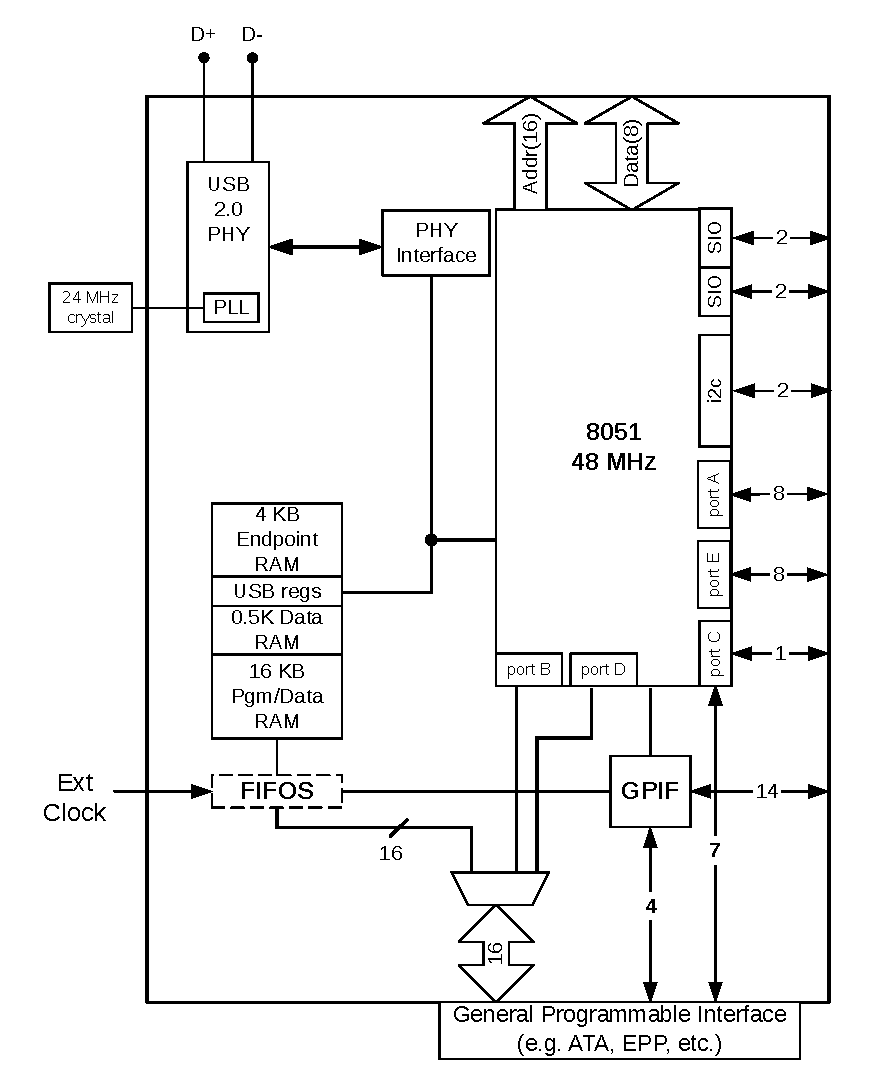
\includegraphics[width=.55\textwidth]{arq.eps}
	\caption{Arquitectura FX2LP~\cite{CypressSemiconductor2014fx2lp}} 
	\label{arqEzUSB}
\end{figure}

La GPIF está pensada principalmente para poder utilizar sistemas que deban ser comandados en forma externa, como por ejemplo un registro de desplazamiento. Por su parte, la memoria FIFO posee \SI{4}{\kilo\byte} de capacidad reservados para almacenar los datos que se intercambian y se destina a aquellos sistemas que pueden proveer las señales de control, aunque también puede ser comandada por el GPIF. Con estas interfaces se posibilita la conexión con casi cualquier dispositivo, ya sea estandarizado (ATA, PCMCIA, EPP, etc) o personalizable (DSP, FPGA, $\mu$C);

%El usuario puede trasmitir datos desde y hacia el Host a través del mismo puerto USB. Sin embargo, también posee dos puertos USART ((acrónimo de Transmisión y Recepción Asíncrona en Serie Universal, en inglés)) que permiten comunicarse con la PC y facilitan en gran medida la tarea de depuración del desarrollo.

%En cuanto a la interfaz con uno o mas periféricos, el controlador posee un puerto $I^2C$, una interfaz de propósito general (GPIF), para sistemas que necesitan ser comandados en forma externa; y una interfaz con memorias FIFO esclavas, a través de las cuales se puede conectar sistemas que cumplen un rol activo en el envío y recepción de información. Estas tres interfaces posibilitan la conexión de dispositivos que poseen tanto puertos estandarizados (ATA, PCMCIA, EPP, etc.), cómo personalizables (DSP, FPGA, microcontroladores, etc).

%Variante 1
 
%El usuario puede trasmitir datos desde y hacia el anfitrión a través del mismo puerto USB, o bien via RS-232. Para comunicarse con sistemas periféricos se puede aprovechar el puerto $I^2C$, la interfaz de propósito general, que actúa como maestro y a la cual se le puede acoplar un periférico esclavo, y/o las memorias FIFO en modo esclavo que puede ser conectada a un sistema maestro. Esto brinda muchas alternativas, desde la conexión a puertos estandar, como ser ATA, PCMCIA, EPP, etc. o también la conexión de dispositivos tales como DSP's y FPGA's.\\
%\textbf{\hl{variante 1}}
%\hl{El usuario puede trasmitir datos desde y hacia el anfitrion a traves del mismo puerto USB, o bien via RS-232. Para comunicarse con sistemas perifericos se puede aprovechar el puerto $I^2C$, la interfaz de proposito general, que actua como maestro y a la cual se le puede acoplar un periferico esclavo, y/o las memorias FIFO en modo esclavo que puede ser conectada a un sistema maestro. Esto brinda muchas alternativas de conexion, desde puertos estandar, como ser ATA, PCMCIA, EPP, etc. hasta dispositivos personalizables como DSP's y FPGA's}.%\\

%variante 2
%El flujo de datos posee dos puntas entre las cuales el controlador hace de nexo. Para ello necesita poder comunicarse tanto con el \host como con los periféricos.\\
%
%El intercambio de información con el \host se lleva a cabo a través del mismo puerto USB, objetivo principal de este trabajo. Sin embargo, también posee dos puertos UART que facilitan en gran medida la tarea de depuración del desarrollo.\\
%
%En cuanto a la interfaz con uno o más periféricos, el controlador posee un puerto $I^2C$, una interfaz de propósito general (GPIF), para sistemas que necesitan ser comandados en forma externa; y una interfaz con memorias FIFO esclavas, a través de las cuales se puede conectar sistemas que cumplen un rol activo en el envío y recepción de información.\\

%\textbf{\hl{variante 2}}
%
%\hl{El flujo de datos posee dos puntas (una PC y un FPGA) entre las cuales el controlador cumple el rol de interfaz. Para ello necesita poder comunicarse tanto con el host como con los perifericos.}%\\
%
%\hl{El intercambio de informacion con el HOST se lleva a cabo a traves del mismo puerto USB, objetivo principal de este trabajo. Sin embargo, tambien posee dos puertos UART que facilitan en gran medida la tarea de depuracion del desarrollo.}%\\
%
%\hl{En cuanto a la interfaz con uno o mas perifericos, el controlador posee un puerto $I^2C$, una interfaz de proposito general (GPIF), para sistemas que necesitan ser comandados en forma externa; y una interfaz con memorias FIFO esclavas, a traves de las cuales se puede conectar sistemas que cumplen un rol activo en el envio y recepcion de informacion.}%\\

Bajo el criterio de este autor, el componente de mayor trascendencia en el funcionamiento del controlador FX2LP es el $\mu$C 8051. Es este componente el encargado de configurar los bloques programables y de inicializar todos los registros que determinan la forma en la que el sistema funciona: la frecuencia de trabajo, la gestión de las memorias y el modo en que fluyen los datos son algunas de las tareas que configura el $\mu$C. El firmware es escrito en lenguaje C para microcontroladores. 

La estructura de la interfaz implementada en este trabajo utiliza la memoria FIFO en modo esclavo, es decir, la memoria responde a señales que proporciona un maestro externo sintetizado en un FPGA. Se escogió la frecuencia de funcionamiento del PLL y se configuraron los extremos que intervienen en la comunicación USB y el modo de funcionamiento, por lo que a continuación se explicitan los detalles referidos a la configuración realizada, con lo que se busca aclarar el funcionamiento y que el lector comprenda los fundamentos de las configuraciones que se plasman en el código del firmware.

\subsection{Microcontrolador Cypress 8051 Mejorado}
	Las tareas que ejecuta el controlador FX2LP son llevadas a cabo por un microcontrolador incorporado al circuito integrado. Dicho $\mu$C es una modificación del 8051 desarrollado por Intel, para que sea más veloz en sus tiempos de ejecución y mejore el desempeño del $\mu$C cómo interfaz, mediante la incorporación de registros especiales adicionales.  De esta forma, la manera a través de la cuál el desarrollador elabora la configuración del controlador, es a través de la programación de este $\mu$C 8051.
	
	Para elaborar el firmware que ejecuta el controlador FX2LP, se desarrolló un programa en C para microcontroladores y se compiló mediante el compilador C51 de Keil, a través del entorno de desarrollo integrado Keil $\mu$Vision. Los archivos resultantes de la configuración realizada se pueden encontrar en el Apéndice~\ref{ap:fx2lp}
	
	Cypress provee, dentro del kit de desarrollo CY3684, un conjunto de archivos que contienen código base sobre el cual el desarrollador implementa la configuración. Este conjunto de archivos es denominado framework, el cual posee, entre otras cosas, encabezados con definiciones de macros, constantes, registros, tipos de datos y declaración de funciones prototipo. También incorpora algunas funciones precompiladas para utilizar los periféricos que contiene la placa de desarrollo.
	
	La Figura \ref{int:fw} muestra un diagrama de flujo del firmware que se desarrolló en el presente trabajo. El mismo fue elaborado utilizando la estructura propuesta por Cypress para el desarrollo de la comunicación que se implementó. Se puede observar que al inicio del programa se inicializan variables de estado que corresponden a una máquina de estados, desarrollada por Cypress, que ejecuta las tareas de la comunicación USB. Luego, se invoca una función llamada \verb|TD_Init()|. Esta es la función a través de la cual se implementa la configuración que se desarrolló en este trabajo. En las secciones siguientes se profundiza cada uno de los bloques que intervienen.
	
	Una vez configurado el funcionamiento del controlador, se habilitan las interrupciones, lo que da lugar a que todos los bloques del circuito integrado puedan funcionar e intercambiar información. Seguidamente, el programa entra en un lazo infinito, donde en primer lugar ejecuta la función \verb|TD_Poll()|, en la cual el desarrollador programa las tareas que ejecuta el controlador durante la rutina de funcionamiento. Como segundo paso, el controlador chequea si arribó desde el Host una transferencia de control cuyo PID indique Setup. En caso afirmativo, ejecuta lo solicitado por el Host. En caso contrario, vuelve a ejecutar la función \verb|TD_Poll()|.
	
	\begin{figure}[h]
	\centering
	\begin{tikzpicture}[scale=.75\textwidth/\paperwidth]
	\begin{scope}[transform shape,node distance=1,>=latex]
	\node[mealy]	(start)	[]	{Iniciar: Reset \\ \verb|main();|};
	\node[moore]	(init)	[below=of start]	{Inicia Variables de Estado}
	edge[<-,thick] (start);
	\node[moore]	(us1)	[below=of init]		{\verb|TD_Init();|}
	edge[<-,thick]	(init);
	\node[moore]	(EI)	[below=of us1]	{Habilita\\Interrupciones}
	edge[<-,thick](us1);
	\node[node distance=0.7]			(aux1)	[below=of EI] 	{};
	\draw[<-,thick](aux1.base) to (EI);
	\node[moore,node distance=.5]	(poll)	[below=of aux1]	{\verb|TD_Poll();|}
	edge[<-,thick](aux1.base);
	\node[ask]		(pr1)	[below=of poll]	{Paquete de Setup}
	edge[<-,thick](poll);
	\node[moore]	(setup)	[right=of pr1]	{\verb|SetupComand();|};
	\draw[->,thick] (setup) |- (aux1.base);
	\node[]			(aux2)	[below=of pr1]	{};
	\draw[->,thick]	(pr1) -- node[above,near start]{Si} (setup);
	\draw[thick]	(pr1) -- node[left,near start]{No}	(aux2.base);
	\node[node distance=2.5](aux3)	[left=of aux2] {};
	\draw[thick]	(aux2.base) -- (aux3.base);
	\draw[->,thick]	(aux3.base)	|-	(aux1.base);
	\end{scope}
	\end{tikzpicture}
	\caption{Diagrama en bloques del firmware que ejecuta el $\mu$C de la interfaz}
	\label{int:fw}
\end{figure}

%	Keil μVision es un entorno de desarrollo integrado (IDE). Se entiende por IDE a un software
%	que integra en un entorno gráfico las herramientas que permiten elaborar un programa que
%	ejecutará un procesador, desde la escritura del algoritmo en uno o más lenguajes, su compilación,
%	las pruebas y el depurado.
%	El programa utilizado posee, entre otras cosas, editor de textos con atajos de teclado,
%	comandos que aceleran la escritura de código y resaltado de palabras claves para diferentes
%	lenguajes de programación, navegador de archivos. También ejecuta, con solo un click, el
%	compilador con la sintaxis correcta, y posee un depurador que, a través de un intérprete, permite
%	ir ejecutando el código lı́nea por lı́nea o en bloques.
%	Para realizar un programa en este entorno, Cypress provee, junto con su framework, un
%	proyecto vacı́o que puede ser copiado y pegado. Sin embargo, se puede realizar la configuración
%	manual. Las instrucciones de este procedimiento se ubican en el Apéndice ??.
%	En cuanto al compilador se refiere, el utilizado es C51. Éste es un programa que otorga
%	un archivo hexadecimal con un código que será ejecutado por microcontroladores que estén
%	implementados con la misma estructura que un Intel 8051, cómo lo es el microcontrolador que
%	posee el FX2LP.
\subsection{Frecuencia de trabajo del sistema}
	La configuración principal del sistema se realiza a través de la función \verb|TD_Init()|. El primer módulo que configura es el PLL ({\it Phase-Locked Loop}). Un PLL es un lazo de servocontrol cuyo parámetro controlado es la fase de una réplica, generada en forma local, de una señal de entrada~\cite{Sklar2001}. En otras palabras, permite obtener dos señales iguales a través de un detector de fase. Si se incorpora un contador entre la señal generada y la entrada del comparador de fase, la señal generada tendrá una frecuencia igual al producto de la entrada por el recorrido del contador. Si, en cambio, se coloca el contador a la salida del PLL, la frecuencia puede ser dividida. Así, es posible obtener señales de frecuencia modificable.

	El PLL incorporado en el controlador permite elevar la frecuencia de un cristal de \SI{24}{\mega\hertz} hasta los \SI{480}{\mega\hertz} que necesita el transceptor USB para el cumplimiento de la norma USB. A su vez, a través de un divisor de frecuencias, permite seleccionar diferentes frecuencias de trabajo del $\mu$C 8051, entre \si{12}, \si{24} o \SI{48}{\mega\hertz}.
	
	A través de los bits especiales CLKSPD[1:0] del registro de Control y Estado de CPU (CPUCS). En la implementación realizada, se seleccionó la frecuencia de trabajo del $\mu$C a \SI{48}{\mega\hertz}.
	
	\begin{lstlisting}[language=C,backgroundcolor=\color{gray!30}]
	//CPUCS - Registro de Control y Estado del CPU
	//	CLKSPD[1:0] -> "00" => 12 MHz
	//				-> "01" => 24 MHz
	//				-> "10" => 48 MHz
	CPUCS = ((CPUCS & ~bmCLKSPD) | bmCLKSPD1); // 48 MHz
	\end{lstlisting}	

\subsection{Memoria FIFO}
	El controlador FX2LP posee una sección especial de memoria destinada al almacenamiento de los datos que fluyen desde cada uno de los extremos de la comunicación. A esta memoria pueden acceder tanto los componentes del propio controlador, como también los periféricos que se comunican a través de él. Desde el punto de vista de la electrónica digital, cada uno de los componentes que acceden a esta memoria pueden tener diferentes fuentes de señal de reloj. Para salvar los inconvenientes que puede acarrear el uso de sistemas con fuentes de reloj independientes, esta porción de memoria reservada es de tipo FIFO. Debido a que se puede acceder a estas memorias FIFO tanto desde el interior de controlador FX2LP, como desde el exterior, deben ser configuradas en ambos sentidos.
	
	La memoria FIFO puede ser programada y configurada de diferentes formas, en función de los requerimientos sistemas periféricos acoplados a ella. Cada uno de los periféricos conectados a la memoria FIFO se denomina extremo o EP\footnote{EP es una abreviación del término inglés {\it endpoint}, que significa ``Extremo''. Esto quiere decir que cada uno de los periféricos conectados a la memoria FIFO es un extremo de la comunicación.}. Las características a configurar son el tamaño (\si{64}, \si{512} o \SI{1024}{\byte}), la cantidad de bloques o partes en que se divide la memoria (puede estar dividida hasta en 4 extremos) y la cantidad de buffers de datos utilizados para almacenar los datos de cada bloque de memoria.
	
	Los buffers son porciones de memoria físicamente separadas pero que, en la operación, el controlador puede intercambiar de forma tal que se acceda a ellos a través de una misma dirección de memoria. El uso de buffers múltiples implica que un EP utiliza más de un buffer. Los buffers múltiples poseen la función de evitar la congestión de datos. Con doble buffer, un periférico coloca o extrae datos del buffer de un EP, mientras el $\mu$C, utiliza otro del mismo EP. La selección del buffer donde cada componente escribe y/o lee los datos lo asigna e intercambia la interfaz en forma automática. Se pueden configurar también un triple o cuádruple buffer, lo que agrega sendas porciones de memoria extra a la reserva. De esta forma, se le otorga al sistema, en forma simultánea, gran capacidad de datos y ancho de banda.
	
	En este desarrollo, se configuró la memoria FIFO con dos EP. El EP2\footnote{EPx será un extremo con dirección x, siendo x un número entero. En este caso, EP con dirección 2.}, es un EP de entrada (envía datos al Host). Requiere una gran cantidad de datos, debido a que será por donde los sensores transmitirán todos los datos que adquieran. Además, es necesario que posea una buena cantidad de almacenamiento de datos y que estos datos sean enviados de la forma más rápida posible. Por tanto, el EP2 se configuró con dos buffers de \SI{1024}{\byte}, para que efectúe transferencias isócronas.
	
	Por su parte, se configura el EP8 como EP de salida (recibe datos desde el Host). Este EP se utiliza para recibir la configuración de los sensores, que se espera que sea de menor cantidad y más distanciada en el tiempo que los datos adquiridos. Se configuró, entonces, con dos buffers de \SI{512}{\byte} para transferencias en masa.
	
	Debido a que la memoria FIFO cumple el rol de interfaz entre los periféricos y el módulo del controlador FX2LP que efectúa las tareas propias de la comunicación USB, la configuración de dicha memoria se efectúa por separado, conteniendo información relevante a cada etapa de la comunicación.
	
\subsubsection{Interfaz hacia los periféricos}
	Cypress provee varias interfaces para comunicar el controlador hacia los periféricos. I$^2$C y UART son dos posibilidades, aunque poseen un ancho de banda muy limitado. La interfaz que opera con mayor ancho de banda es la memoria FIFO. Esta puede ser utilizadas en modo esclavo, es decir, que un sistema externo comande la lectura y la escritura de datos en ellas, o bien, a través de la interfaz GPIO, puede ser comandada por el $\mu$C 8051. La implementación que se realiza en el desarrollo de la comunicación utiliza la memoria FIFO en modo esclavo.
	
	La frecuencia de funcionamiento de estas interfaz es independiente del reloj del sistema. Puede ser configurado para usar una señal de reloj interna de \si{30} o \SI{48}{\mega\hertz}, propia de la interfaz, o bien, ser provista por un sistema externo al controlador. También, es importante indicarle al controlador si la interfaz funcionará en modo asíncrono. Todos estos parámetros son configurados a través del registro Configuración de Interfaz (IFCONFIG).
	
	La configuración que se realizó en esta implementación, utiliza el reloj interno de la interfaz, corriendo a \SI{48}{\mega\hertz}. Además, se indica que las memorias FIFO esclavas son utilizadas en modo asincrónico. Dicha configuración se plasma en las siguientes líneas de código:
	
	\begin{lstlisting}[language=C,backgroundcolor=\color{gray!30}]
	//IFCONFIG - Registro de Configuración de la Interfaz
	//	b7 	   -> fuente de reloj: '1' interna, '0' externa
	//	b6 	   -> frec: '1' 48 Mhz, '0' 30 MHz
	//	b3 	   -> asinc: '1' asíncrono
	//	b[1:0] -> modo de interfaz: "11" FIFO esclava
	IFCONFIG = 0xCB;
	SYNCDELAY;
	\end{lstlisting}

	El controlador FX2LP posee cuatro pines que emiten señales del estado de las memorias FIFO (comunmente conocidas como ''banderas´´ o \textit{flags}). Dichos pines pueden ser programados para que indiquen si una porción particular de memoria se encuentra vacía, llena o si sobrepasa un nivel programable de datos. También pueden ser configurados para que indiquen el estado completo (vacío, lleno y el nivel programable) de la porción de memoria activa. Cada porción de memoria se activa a través de dos puertos de dirección, comandados por un sistema externo al controlador FX2LP.
	
	Para la comunicación desarrollada, solo son importantes las banderas que indican cuando el EP8 está vacío y que el EP2 está lleno. Si bien no son necesarias, por completitud, también se configuraron las señales que indican que el EP2 está vacío y que el EP8 se encuentra lleno. Cada uno de los \textit{flags} se denominan A, B, C y D y se configuran por pares a través de los registros PINFLAGSAB y PINFLAGSCD, de la forma en que se muestra a continuación.
	
	\begin{lstlisting}[language=C,backgroundcolor=\color{gray!30}]
	PINFLAGSAB = 0xBC;	// FLAGA <- EP2 Full Flag
						// FLAGD <- EP2 Empty Flag
	SYNCDELAY;
	PINFLAGSCD = 0x8F;	// FLAGC <- EP8 Full Flag
						// FLAGB <- EP8 Empty Flag
	\end{lstlisting}
	
	
\subsubsection{Interfaz hacia el módulo de comunicación USB}
	Desde el extremo interno del controlador FX2LP, la memoria FIFO se conecta al Motor de Interfaz Serial (MIS). El MIS es un módulo que se encarga de tomar datos en paralelo y convertilos en una secuencia seriada. Para cumplir con la norma USB, el MIS debe ser capaz de empaquetar, enviar, recibir y desempaquetar toda la información, así como leer los Token que emite el Host, calcular y corroborar los códigos cíclicos de detección de errores y todo lo relacionado al protocolo propiamente dicho. Luego, el transceptor USB efectúa las tareas de codificación y decodificación de los mensajes transmitidos a través del bus.
	
	Para la configuración, es necesario indicarle al controlador FX2LP el funcionamiento que tendrá cada uno de los EP. Los parámetros programables son: si está activo o no, el sentido de la comunicación (sea hacia o desde el Host), el tipo de transferencia, el tamaño de la misma y la cantidad de buffers múltiples que se utilizan. En el desarrollo que se presenta se configura el EP2 como entrada de \SI{1024}{\byte} con dos buffers y el EP8 como salida con dos buffers de \SI{512}{\byte}. También se configura el EP1 con un buffer de \SI{64}{\byte} como entrada y otro igual como salida, ya que viene implementado en una memoria separada dentro del circuito integrado FX2LP y no interfiere con el desempeño pretendido en este trabajo. Los otros EP válidos (EP4 y EP6) no se utilizan, con el objetivo de maximizar la memoria disponible para los datos útiles. De esta forma, la configuración se realiza a través de la siguiente línea de código:
	
	\begin{lstlisting}[language=C,backgroundcolor=\color{gray!30}]
	//EPxCFG - Registros de configuración de extremos
	//	b7 	   -> '1' EP activo
	//	b6 	   -> dir: '0' salida, '1' entrada
	//	b[5:4] -> tipo: "01" => isocronico
	//					"10" => masa
	//					"11" => interrupción
	//	b3 	   -> tamaño: '0' 512 bytes, '1' 1024 bytes
	//	b[1:0] -> buffer: 	"00" => x4
	//						"10" => x2
	//						"11" => x3
	EP1OUTCFG = 0xA0;
	SYNCDELAY;
	EP1INCFG = 0xA0;
	SYNCDELAY;
	// dir:entrada, tipo:isoc, tam:1024, x3
	EP2CFG = 0xDB;
	SYNCDELAY;
	EP4CFG = 0x7F; //Inactivo
	SYNCDELAY;
	EP6CFG = 0x7F; //Inactivo
	SYNCDELAY;
	// dir:salida, tipo:masa, tam:512, x2
	EP8CFG = 0xA2; 
	SYNCDELAY;
	\end{lstlisting}
	
%\subsection{Motor de Interfaz Serial}
%	El Motor de Interfaz Serial (MIS) es un módulo incorporado al circuito integrado que se encarga de tomar datos en paralelo y convertilos en una secuencia seriada.

%	\begin{figure}[ht]%TODO hacer con tikz para que quede prolija
%		\centering
%		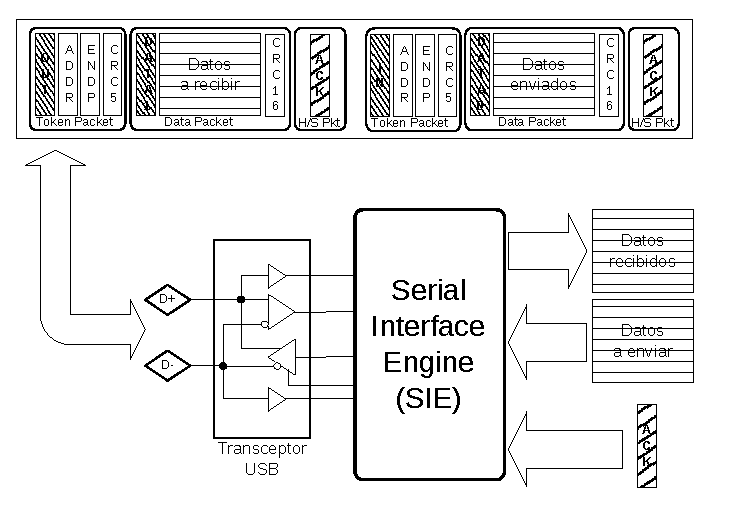
\includegraphics[width=.8\textwidth]{usbxcvr}
%		\caption{Implementación del enlace USB realizado por el EZ-USB~\cite{CypressSemiconductor2014fx2lp}}%TODO(\hl{se copiaria con tikz para mejorar prolijidad})}
%		\label{usbxcvr}
%	\end{figure}
%	
%	La comunicación USB entre el controlador FX2LP y la PC se realiza a través del transceptor, unido al MIS. Para realizar el intercambio de datos, el firmware solo debe colocar o extraer los datos de buffers programables y modificar las banderas de handshaking. En forma automática, el MIS se encargan de empaquetar, enviar, recibir y desempaquetar toda la información, así como leer los tokens que emite el host, calcular y corroborar los códigos cíclicos de detección de errores y todo lo relacionado al protocolo propiamente dicho. El transceptor codifica y decodifica todo a nivel físico.%\\
%	
%	La Figura \ref{usbxcvr} muestra la función del MIS. Toma los datos colocados en los buffers de extremos, agrega la información que corresponde al encabezado y a la cola y, finalmente, coloca el registro de handshaking. Esto último, se observan como ACK (abreviación del ingles {\it acknowledge}, que significa reconocer, aceptar o agradecer) en la Figura \ref{usbxcvr}. En el extremo del controlador, estas banderas se colocan en un registro especial que indica si el sistema está disponible, si los datos fueron colocados o leídos, dependiendo el caso tratado.

%\subsection{Modo}		
%\subsection{Buffers de extremos}
%	El MIS guarda los datos que aún no han sido enviados y/o los que han sido recibidos pero no leídos por ningún periférico en una memoria RAM específica, denominada buffer de extremo.%\\
%	
%	La norma USB define a un dispositivo extremo como una porción exclusiva e identificable de una dispositivo USB que es fuente o un sumidero de información. En otras palabras, USB ve a cada extremo como una memoria FIFO de donde surge o finaliza la información. En ingles, el termino extremo recibe el nombre de {\it endpoint}, por lo que, en adelante, cuando se hable de ellos se abreviara como EP o EPx, siendo la x un número que indica la dirección del extremo.%\\
%	
%	La serie de controladores FX2LP dispone de hasta 7 EP programables, los cuales deben poseer al menos dos buffers. La norma USB indica que cualquier dispositivo USB debe poseer un EP con dirección 0 que se destina para control y configuración, por lo que el controlador está dotado de \SI{64}{\byte} para este fin. Es el único EP que puede ser bidireccional en el sentido del flujo de datos. A través de él, host y dispositivo envían y reciben transferencias de control. Luego, se incorporan dos EP1, que poseen un buffer de \SI{64}{\byte} cada uno. Estos EP se identifican por la dirección de los datos, ya que uno de ellos es de salida y el otro de entrada de datos.%\\
%	
%	\begin{figure}[t]
%		\centering
%		\begin{tikzpicture}[scale=.7*\textwidth/\paperwidth,node distance=2.7]
%			\begin{scope}[transform shape]
%				\begin{scope}[node distance=0.4]
%					\node[buf]	(ep2b1)	[anchor=north]		{\ep{1}{2}{512}};
%					\node[buf]	(ep2b2)	[below=of ep2b1]	{\ep{2}{2}{512}};
%					\node[obuf]	(ep4b1) [below=of ep2b2]	{\ep{1}{4}{512}};
%					\node[buf]	(ep4b2) [below=of ep4b1]	{\ep{2}{4}{512}};
%					\node[obuf]	(ep6b1)	[below=of ep4b2]	{\ep{1}{6}{512}};
%					\node[buf]	(ep6b2)	[below=of ep6b1]	{\ep{2}{6}{512}};
%					\node[obuf]	(ep8b1)	[below=of ep6b2]	{\ep{1}{8}{512}};
%					\node[buf]	(ep8b2)	[below=of ep8b1]	{\ep{2}{8}{512}};
%				\end{scope}
%				
%				\begin{scope}[node distance=0.4, xshift=90]
%					\node[buf]	(ep2b3)	[anchor=north]		{\epg{1}{2}{1024}};
%					\node[obuf] (ep2b4)	[below=of ep2b3]	{\epg{2}{2}{1024}};
%					\node[obuf]	(ep2b5)	[below=of ep2b4]	{\epg{3}{2}{1024}};
%					\node[obuf]	(ep8b3)	[below=of ep2b5]	{\ep{1}{8}{512}};
%					\node[buf]	(ep8b4)	[below=of ep8b3]	{\ep{2}{8}{512}};
%				\end{scope}
%			\end{scope}
%		
%			\begin{scope}[on background layer]
%				rounded corners,]
%				\node[env, fit=(ep2b1)(ep2b2)]			(ep21)	{};
%				\node[env, fit=(ep4b1)(ep4b2)]			(ep41)	{};
%				\node[env, fit=(ep6b1)(ep6b2)]			(ep61)	{};
%				\node[env, fit=(ep8b1)(ep8b2)]			(ep81)	{};
%				\node[env, fit=(ep2b3)(ep2b4)(ep2b5)]	(ep22)	{};
%				\node[env, fit=(ep8b3)(ep8b4)]			(ep82)	{};
%				\node[draw=black,fit=(ep21)(ep82)](marco){};
%			\end{scope}
%		
%			\begin{scope}[transform shape]
%				\draw (marco.north) to (marco.south);
%				\node[left=of ep2b1.north east,anchor=north east](add1)	{0xF000};
%				\node[left=of ep2b1.south east,anchor=south east](add2)	{0xF1FF};
%				\node[left=of ep2b2.north east,anchor=north east](add3)	{0xF200};
%				\node[left=of ep4b1.north east,anchor=north east](add4)	{0xF400};
%				\node[left=of ep6b1.north east,anchor=north east](add5)	{0xF800};
%				\node[left=of ep8b1.north east,anchor=north east](add6)	{0xFC00};
%				\node[left=of ep8b2.south east,anchor=south east](add7)	{0xFFFF};
%				\draw[dashed] (add1.north west) to (add1.north west -| marco.east);
%				\draw[dashed] (add3.north west) to (add3.north west -| ep21.east);
%				\draw[dashed] (add4.north west) to (add4.north west -| marco.east);
%				\draw[dashed] (add5.north west) to (add5.north west -| marco.east);
%				\draw[dashed] (add6.north west) to (add6.north west -| marco.east);
%				\draw[dashed] (add7.south west) to (add7.south west -| marco.east);
%			\end{scope}
%	\end{tikzpicture}
%	\caption{Buffers de extremos con sus direcciones de memoria. El cuadro de la izquierda muestra la configuración por defecto. El derecho, la implementada en este trabajo.}
%	\label{epbuf}
%	\end{figure}
%	
%	Finalmente, se incorpora una memoria de \SI{4}{\kibi\byte} que debe ser configurada para los EP2, EP4, EP6 y EP8. La configuración de los EP la realiza el microcontrolador una vez que su programa se encuentra en ejecución. Las variables, conforme a los requerimientos de ancho de banda y acceso al bus son:
%	
%	\begin{itemize}
%		\item Tamaño: Dependiendo del extremo a configurar puede ser de 512 o 1024 bytes.
%		\item Tipo de acceso al bus: Definido según la norma USB, este tipo puede ser por bultos, isócrono o de interrupción. No se admiten en estos EP paquetes de control.
%		\item Cantidad de buffers: Dependiendo del extremo, puede ser dos, tres o cuatro buffers por extremo.
%		\item Habilitación: Se debe indicar al sistema si los extremos se usan o no. El EP no valido, no responderá a un pedido de entrada o salida.
%	\end{itemize}
%	
%	La Figura \ref{epbuf} muestra solo dos de las posibles configuraciones de los EP. A la izquierda se observa la configuración por defecto del controlador FX2LP. Esto es, los cuatro EP habilitados, con 512 bytes cada uno, buffers dobles y comunicación por bultos. A la derecha se muestra la configuración elegida para este trabajo, es decir, solo son EP válidos el EP2 y EP8. EP2 posee tres buffers de 1024 bytes y el EP8 dos buffers con 512 bytes de capacidad cada uno. Siempre se debe considerar que se dispone hasta \SI{4}{\kibi\byte} de memoria.%\\
%	
%	La característica de los buffers múltiples evita la congestión de datos. Con doble buffer, un periférico (o el microcontrolador) coloca o extrae datos de un buffer, mientras otro, del mismo EP, se encuentra enviando o recibiendo datos mediante el MIS. Cuando se configura un triple o cuádruple buffer, se agrega una o dos porciones mas de memoria a la reserva, respectivamente. De esta forma, se le otorga al sistema una gran capacidad de datos y ancho de banda.%\\
%	
%	Un detalle importante de los buffers múltiples es que, a la vista del controlador y/o de un periférico, el buffer posee una sola y única dirección y, es la propia interfaz FX2LP quien se encarga de seleccionar el buffer que corresponde en cada caso. Esto quiere decir que, por ejemplo, teniendo 4 buffers de \SI{512}{\byte} cada uno, el 8051 verá solo uno de \SI{512}{\byte}, sin necesidad de identificar a traves de su firmware con cuál de los cuatro está trabajando.
%	
%\subsection{Memorias FIFO esclavas}
%	\label{cy:fifo}
%	Desde el punto de vista de la electrónica digital, el MIS es un dispositivo que recibe y envía datos desde y hacia el puerto USB utilizando una señal de reloj de \SI{24}{\mega\hertz}. Esta señal, es provista por un cristal de cuarzo incorporado en el circuito impreso del Kit de Desarrollo CY3684 EZ-USB FX2LP. Por su parte, un sistema externo puede o no proveer una señal de reloj y manejo de datos propio cuy a fuente de reloj es a priori desconocida por quien configura el circuito integrado. El controlador USB incorpora memorias FIFO que se encargan de proveer una interfaz entre el MIS y un dispositivo externo, salvando el problema de poseer dos relojes diferentes e independientes.%\\
%	
%	Estas memorias funcionan en modo esclavo, es decir, se debe conectar un dispositivo capaz de proveer una lógica maestra externa que comande la entrada y salida de datos desde una memoria FIFO hacia o desde el exterior. Para los fines del presente trabajo, este modo de funcionamiento es óptimo ya que, dotando al FPGA de una máquina de estados, se logra la transferencia de datos en los tiempos requeridos.%\\
%	
%	El sistema de bus permite conectar a estas memorias hasta cuatro dispositivos diferentes. Por esto, existe un registro que permite seleccionar una porción de memoria FIFO para cada uno de los EP programables en el buffer de extremos.%\\
%	
%	\begin{figure}[ht]
%		\centering
%		\begin{tikzpicture}[scale=1*\textwidth/\paperwidth]
%			\begin{scope}[transform shape,node distance=4,>=latex]
%				\node[simple]	(fifo)		[]	 			{FIFO's Esclavas};
%				\node[simple]	(master)	[right=of fifo]	{Maestro Externo};
%				\draw[<->,thick]	([yshift=5*110/6]fifo.east) --node [above]{IFCLK} ([yshift=5*110/6]master.west);
%				\draw[<->,thick]	([yshift=4*110/6]fifo.east) --node [above]{FD[15:0]} ([yshift=4*110/6]master.west);
%				\draw[<-,thick]	([yshift=3*110/6]fifo.east) --node [above]{FIFOADR[1:0]} ([yshift=3*110/6]master.west);
%				\draw[->,thick]	([yshift=2*110/6]fifo.east) --node [above]{FLAGA} ([yshift=2*110/6]master.west);
%				\draw[->,thick]	([yshift=1*110/6]fifo.east) --node [above]{FLAGB} ([yshift=1*110/6]master.west);
%				\draw[->,thick]	([yshift=0*110/6]fifo.east) --node [above]{FLAGC} ([yshift=0*110/6]master.west);
%				\draw[->,thick]	([yshift=-1*110/6]fifo.east) --node [above]{FLAGD} ([yshift=-1*110/6]master.west);
%				\draw[<-,thick]	([yshift=-2*110/6]fifo.east) --node [above]{SLOE} ([yshift=-2*110/6]master.west);
%				\draw[<-,thick]	([yshift=-3*110/6]fifo.east) --node [above]{SLWR} ([yshift=-3*110/6]master.west);
%				\draw[<-,thick]	([yshift=-4*110/6]fifo.east) --node [above]{SLRD} ([yshift=-4*110/6]master.west);
%				\draw[<-,thick]	([yshift=-5*110/6]fifo.east) --node [above]{PKTEND} ([yshift=-5*110/6]master.west);
%			\end{scope}				
%		\end{tikzpicture}
%		\caption{Puertos de interfaz entre las FIFO's y un maestro externo}
%		\label{interfazfifo}
%	\end{figure}
%
%	La Figura \ref{interfazfifo} muestra las señales de la interfaz entre las memorias FIFO's y un maestro esclavo. Estas son:
%	
%	\begin{itemize}
%		\item IFCLK: señal de reloj. No es necesario en caso de conectar la interfaz en modo asincrónico. La señal de reloj puede ser provista por el controlador o por el dispositivo de control en forma programable.
%		\item FD[15:0]: constituye el bus de datos. Según se programe, este puede ser de 8 o 16 bits, en forma independiente para cada EP.
%		\item FIFOADDR[1:0]: puerto de direcciones. A través de él se selecciona la memoria activa en el bus.
%		\item FLAGx: Los cuatro puertos de flag son configurables e indican memoria llena, vacía o un nivel programable. También pueden indicar el estado de una memoria específica o de la que se encuentra activa a través de FIFOADDR.
%		\item SLOE, SLWR, SLRD: son las señales de control. A través de ellas el maestro entrega las ordenes de lectura y escritura.
%		\item PKTEND: a través de este puerto el maestro indica que terminó una transferencia de datos.
%	\end{itemize}

\subsection{Modos de entrada y salida automáticos}
	
	Los datos se reciben o envían a través del MIS. Dichos datos, pueden ser enviados en forma automática desde y hacia las memorias FIFO, o bien, pueden ser dirigidos hacia el $\mu$C, el cual debe dirigir los datos desde y hacia su destino (el MIS o las memorias). Esto último permite leer, modificar, suprimir, agregar y/o generar nuevos datos antes de ser remitidos a su destinatario. Estos caminos se pueden ver en la Figura \ref{modesfifo}.%\\
	
	Aunque el envío de datos se hace siempre de forma automática, el fabricante llama a estos caminos "MODO MANUAL", en caso de enviar los datos a través del $\mu$C 8051, y "MODO AUTOMÁTICO", cuando la comunicación es directa entre el MIS y las FIFO. Además, se programan en forma independiente para cada extremo, sea este de salida o entrada. Es decir, la entrada de un EP puede ser manual y la entrada de otro puede ser automática.%\\
	
	Se debe notar en la Figura \ref{modesfifo} que se refiere a paquetes de entrada cuando estos poseen una dirección que se inicia en un periférico y termina en el host y de salida cuando llevan el sentido contrario. Esto se debe al rol central que ejerce el host en la comunicación USB.
	
	\begin{figure}[b]
		\centering
		\begin{tikzpicture}[scale=0.8\textwidth/\paperwidth,text width=5em,align=center,>=latex,node distance=38mm]		
			\begin{scope}[transform shape]
				\node[interior]	(mis)									{MIS};
				\node			(im)	[right=of mis]					{};
				\node[interior]	(uc)	[above=of im]					{$\mu$C};
				\node[interior] (fifo)	[right=of im,text width=4em]	{FIFOs Esclavas};
				\node			(et)	[left=of uc]					{FX2LP};
				
				\draw[->]([xshift=1.5mm]fifo.north)to node[above,mode text]{MODO ENTRADA MANUAL} ([yshift=1mm]uc.east);
				\draw[->]([yshift=1mm]uc.west)to node[above,mode text]{MODO ENTRADA MANUAL}([xshift=-1.5mm]mis.north);
				\draw[->] ([yshift=-1mm]uc.east)to node[below,mode text]{MODO SALIDA MANUAL}([xshift=-1.5mm]fifo.north);
				\draw[->]([xshift=1.5mm]mis.north)to node[below,mode text]{MODO SALIDA MANUAL}([yshift=-1mm]uc.west);
				
				\draw[->]([yshift=1mm]fifo.west)to node[above,mode text]{MODO AUTO ENTRADA}([yshift=1mm]mis.east);
				\draw[->]([yshift=-1mm]mis.east)to node[below,mode text]{MODO AUTO SALIDA}([yshift=-1mm]fifo.west);
				
				\node[exterior]	(pc)	[left=of mis]	{Host};
				\draw[->]([yshift=1mm]mis.west)to([yshift=1mm]pc.east);
				\draw[->]([yshift=-1mm]pc.east)to([yshift=-1mm]mis.west);
				
				\node[exterior]	(fpga)	[right=of fifo]	{Maestro Externo};
				\draw[->]([yshift=1mm]fifo.east)to node[above]{Banderas}([yshift=1mm]fpga.west);
				\draw[<-]([yshift=-1mm]fifo.east)to node[below]{Control}([yshift=-1mm]fpga.west);
				\end{scope}	
				
				\begin{scope}[on background layer]
				\node(fx)[rounded corners,fill=black!10,fit=(mis)(uc)(fifo)(et)]{};
			\end{scope}
		\end{tikzpicture}
		\caption{Modos de conexión de la memoria FIFO, el microntrolador y el MIS}
		\label{modesfifo}
	\end{figure}

	Para efectuar la configuración del modo de funcionamiento de cada EP, se recurre a los Registros de Configuración Extremo-FIFO esclava (EPxFIFOCFG). A continuación se muestra la programación efectuada en este trabajo, en donde se envían los datos en forma automática, tanto de entrada como de salida. Se debe notar que la activación del modo automático se produce por el flanco ascendente de la variable de configuración, por lo que primero se coloca el registro en cero y luego se establece el valor de la configuración. También se indica en este registro que los datos tendrán un ancho de 16 bits.
	
	\begin{lstlisting}[language=C,backgroundcolor=\color{gray!30}]
	//EPxFIFOCFG - Registro de configuracion extremo/FIFO
	//	b6	->	'1' Indica lleno un byte antes
	//	b5	->	'1' Indica vacío un byte antes
	//	b4	->	'1' Modo Auto Salida
	//	b3	->	'1' Modo Auto Entrada
	//	b2	->	'1' Permite paquetes de entrada con largo 0
	//	b0	->	'1' bus de 16 bits, '0' bus de 8 bits
	EP8FIFOCFG = 0x00;
	SYNCDELAY;
	EP2FIFOCFG = 0x00;
	SYNCDELAY;
	
	//establecer modo auto. se necesita flanco ascendente
	EP8FIFOCFG = 0x11;
	SYNCDELAY;
	EP2FIFOCFG = 0x0D;
	SYNCDELAY;
	\end{lstlisting}
	
	Una vez configuradas las interfaces, se deben restablecer las memorias FIFO, a fin de asegurarse que se encuentran vacías para iniciar la comunicación, a través del registro FIFORESET. El bit 7 de este registro le indica al MIS que la memoria FIFO no se encuentra disponible, y el MIS, a su vez, lo indica al Host si es necesario. Luego, a través de los cuatro bits menores se indica la dirección del EP a restablecer. Finalmente, libera la memoria y se le indica la situación al MIS.
	
	\begin{lstlisting}[language=C,backgroundcolor=\color{gray!30}]
	//FIFORESET - Registro de restablecimiento FIFO
	//	b8		->	'1' Desabilitado
	//	b[3:0]	->	'1' Direccfión de EP
	FIFORESET = 0x80;
	SYNCDELAY;
	FIFORESET = 0x82;
	SYNCDELAY;
	FIFORESET = 0x84;
	SYNCDELAY;
	FIFORESET = 0x86;
	SYNCDELAY;
	FIFORESET = 0x88;
	SYNCDELAY;
	FIFORESET = 0x00;
	SYNCDELAY;
	//establecer modo auto. se necesita flanco ascendente
	EP8FIFOCFG = 0x11;
	SYNCDELAY;
	EP2FIFOCFG = 0x0D;
	SYNCDELAY;
	\end{lstlisting}
	

	En las líneas de código mostradas hasta acá se utiliza el macro {\it SYNCDELAY}. Dicho macro es una secuencia de espera requerida por Cypress para cumplir con los tiempos de mantenimiento asociados a la escritura y lectura de determinados registros~\cite{CypressSemiconductor2014fx2lp}.%, los cuales se explicitan en el Anexo \ref{an:syncdelay}.

	\chapter{Desarrollo del sistema maestro para la comunicación entre la FPGA y la interfaz Cypress}
	\section{Descripción del sistema desarrollado}
		Para el logro de los objetivos del presente trabajo, que es la realización de una comunicación USB para el envío y recepción de información originada en desarrollos científicos basados en un FPGA, es necesario no solo la elaboración de drivers, interfaz y periféricos, sino también un núcleo de FPGA capaz de comunicarse con ambos lados de la interfaz, es decir, con el controlador USB y con el desarrollo mismo, implementado dentro de la FPGA.\\

\begin{figure}
	\centering
	\begin{tikzpicture}[scale=1.4*\textwidth/\paperwidth,>=latex,node distance=3]
		\begin{scope}[transform shape,node distance=1.5,align=center]
		\node[interior,text width=60](mea)	{M\'aquina de Estados Algorítmica};
		\node	(aux1)	[right=of mea]	{};
		\node[interior,text width=60](dev)		[right=of aux1]	{Desarrollo científico};
		\draw[<->] (mea.east) -- node[above]{Flujo de Datos} (dev.west);
		\node[node distance = .5]	(texto fpga) [below=of aux1] {FPGA};
		\end{scope}
		\begin{scope}[on background layer]
		\node[fit=(mea)(dev)(texto fpga),rectangle,draw](fpga){};
		\end{scope}
		\begin{scope}[transform shape,]
		\node[exterior,text width=70,align=center,minimum height=65] (cy)	[left=of fpga]{Controlador FX2LP};
		\end{scope}
		
		\begin{scope}[transform shape]
		\draw[<->] (cy.20) to node[above]{Datos} (cy.20 -| fpga.west);
		\draw[<->] (cy.-20) to node[above] {Control} (cy.-20 -| fpga.west);
		\end{scope}

	\end{tikzpicture}
	\caption{\hl{alguna descripcion}}
	\label{interfaz:ov}
\end{figure}

La Figura \ref{interfaz:ov} muestra un esquema en el cual se observan, como extremos, un desarrollo científico particular y el controlador de Cypress. Entre ambos, se encuentra una Máquina de Estados Algorítmica (MEA) que hace de nexo. La MEA debe poder manejar correctamente las señales de control, así como envíar, recibir y canalizar los datos que circulan a través de ella.\\

La MAE se desarrolla en VHDL y se implementa en la placa MOJO que, cómo se menciona en el Capítulo%TODO referencia al capítulo
, posee una FPGA Spartan VI de Xilinx.\\

Para poder elaborar la MAE, es necesario conocer y entender el funcionamiento y las señales que requiere la interfaz de las memorias FIFO del controlador FX2LP.\\

Por ello, en este capítulo se desarrolla, en primer lugar la estructura de la interfaz. Luego, se aborda el diseño de la MAE y finalmente, su implementación en VHDL.\\

Además de lo anterior, se detalla el diseño y la elaboración de un circuito impreso de interconexión, a través del cual las señales de las placas de desarrollo MOJO y CY3684 conectan en forma física sus puertos.\\

	\section{Señales de Control}
		En el Capitulo \ref{cap:cy} del presente informe se describen los puertos de la interfaz entre un maestro esterno y las memorias FIFO del controlador de Cypress.\\

Al abordar, ahora, el control del mismo, es necesario desarrollar con mayor detalle cada una de estas señales. Así, se podrá comprender, con mayor detalle, las señales que debe enviar y recibir una MEA que controle esta interfaz.\\

Si bien el modo de funcionamiento de la interfaz puede ser síncorno o asíncorno, se detalla sólo este último, es decir, el implementado, ya que debido a errores de diseño de quien escribe, no es posible implementar, hasta el momento de la escritura, un funcionamiento sincrónico del sistema.\\

Por lo anterior, no se detalla en ningún momento la señal del puerto IFCLK.\\

\subsection{Lectura de datos desde la interfaz}

	\begin{figure}
		\centering
		\begin{tikzpicture}[scale=1.4\textwidth/\paperwidth]
			\begin{scope}[transform shape,node distance=1,text width=60]
				\setcounter{wavecount}{0}
				\newwave{FIFOADR[0]}
					\bit{1}{7}
				\newwave{FIFOADR[1]}
					\bit{1}{7}
				\newwave{FLAG Vac\'io}
					\bit{1}{5}
					\bit{0}{2}
				\newwave{SLOE}
					\bit{1}{1}
					\bit{0}{5}
					\bit{1}{1}
				\newwave{SLRD}
					\bit{1}{2}
					\bit{0}{1}
					\bit{1}{1}
					\bit{0}{1}
					\bit{1}{2}
				\newwave{FD[0:15]}
					\bitvector{Z}{1}
					\bitvector{1}{2}
					\bitvector{0}{2}
					\bitvector{X}{1}
					\bitvector{Z}{1}
			\end{scope}
			\begin{scope}[on background layer]
				\foreach \x in {1,2,...,7}{
					\draw[dashed,black!20] (\x.3,0) -- (\x.3,\value{wavecount}+1);}
			\end{scope}
		\end{tikzpicture}
		\caption{este texto}
		\label{if:label}
	\end{figure}

	\section{Máquina de Estados Algorítmica}
		A modo conceptual, la maquina de estados algorítmica (MAE) que se implementa en este trabajo es capaz de realizar dos tareas, bien definidas: leer y escribir datos desde y en la memoria FIFO. En la Figura \ref{fpga:mea:concepto} se muestra que cuando la memoria FIFO señala que no está vacía, se ejecuta la tarea de lectura de datos. Si la memoria FIFO se encuentra vacía y está activa la salida de datos, estos datos serán escritos en la memoria FIFO correspondiente.

Se puede notar que la implementación de estas tareas le otorga mayor prioridad a la operación de lectura que a la de escritura. Es decir, siempre que existan datos para leer en la memoria FIFO, serán leídos, aún cuando hayan datos para ser escritos.
Esta prioridad, viene dada en función de que se prevé que la comunicación sea utilizada por sensores que adquieren datos y los transmiten en forma inmediata a la PC y, a su vez, desde la PC se envía en forma ocasional datos que permitan configurar parámetros del sensor en particular. Por este motivo, se espera que los datos que provengan de la PC sean menos probables que los de los datos que está adquiriendo el sensor.

\begin{figure}[ht]
	\centering
	\begin{tikzpicture}[scale=.7]
		\begin{scope}[transform shape,node distance=3,>=latex,looseness=1.2]
			\node[chart](inicio){En espera};
			\node[chart](lectura)[below left=of inicio]{Leer datos};
			\node[chart](escritura)[below right=of inicio]{Escribir datos};
			\draw[->] (escritura.120) to [bend left](inicio.330);
			\draw[->] (lectura.60) to [bend right](inicio.210);
			\draw[->] (inicio.160) to [bend right] node [above,sloped] {FIFO Vacía=0} (lectura.110);
			\draw[->] (inicio.20) to [bend left] node [above,sloped,text width=80] {FIFO Vacía=1\\Salida datos=1} (escritura.70);
			\draw[->] (inicio.135) to [out=90,in=100,looseness=1.5] node [above,text width=80] {FIFO Vacía=1\\Salida datos=0} (inicio.45);
		\end{scope}
	\end{tikzpicture}
	\caption{Diagrama conceptual de la MEA}
	\label{fpga:mea:concepto}
\end{figure}

La Figura \ref{fpga:variables} muestra un esquema en donde se observan las variables que intervienen en la implementación del sistema. Como se observa en dicha figura, desde el extremo que se comunica con el controlador, las variables de entrada para la operación de lectura son el bus de datos {FD[15:0]\it} y el {\it FLAG Vacío}, conforme al diagrama temporal de la Figura \ref{fpga:lecfifo} En el caso de la operación de lectura, se utiliza además el {\it FLAG Vacío}. Las de salida son los puertos de dirección {\it FIFOADR[1:0]}, SLRD y SLOE para la operación de lectura y se agrega SLWR para la escritura.

\begin{figure}[ht]
	\centering
	\begin{tikzpicture}
		\begin{scope}
		\end{scope}
	\end{tikzpicture}
	\caption{esta figura}
	\label{fpga:variables}
\end{figure}

En la interfaz que se comunica con el interior del FPGA, existen las señales para enviar datos, los datos a enviar, los datos recibidos y una señal que indica que hay datos por recibir. 

Con base en los diagramas temporales y las variables anteriormente mencionadas, se plantea la maquina de estados que se observa en la Figura \ref{fpga:mea}.

\begin{figure}[ht]
	\centering
	\begin{tikzpicture}[ask/.style = {diamond,text width=70,draw=black,align=center,aspect=2},
	scale=.7]
		\begin{scope}[transform shape,node distance=1,>=latex,]
			\node[moore,text width=100] (inicio) [label=above right:inicio]{FIFOADR=$''$ZZ$''$\\SLOE=$'1'$\\SLRD=$'1'$\\SLWR=$'1'$};
			
			\node[ask] (vacio1) [below=of inicio]{FLAG Vacío};
			\draw[->] (inicio.south) -| (vacio1);
			%			\node[moore,text width=100] (lecdir) [below=of vacio1,label=above right:dirección] {FIFOADR=entrada\\SLOE=$'0'$\\SLRD=$'1'$\\SLWR=$'1'$};
			%			\draw[o->](vacio1.east) -- ($(vacio1.east)+(1,0)$);
			
			\node[moore,text width=100] (lecoe) [right=of vacio1,label=above right:dirección] {FIFOADR=entrada\\SLOE=$'0'$\\SLRD=$'1'$\\SLWR=$'1'$};
			\draw[->] (vacio1.east) -- ($(vacio1.east)!0.5!(lecoe.west)$);
			\draw[->]($(vacio1.east)!0.5!(lecoe.west)$) |- ($(lecoe.north)+(0,0.5)$) -- (lecoe.north);
			
			\node[moore,text width=100](lecrd)[below=of lecoe,label=above right:lectura]{FIFOADR=entrada\\SLOE=$'0'$\\SLRD=$'0'$\\SLWR=$'1'$};
			\draw[->](lecoe) -- (lecrd);
			
			\node[ask] (vacio2)[below=of lecrd]{FLAG Vacío};
			\draw[->](lecrd) -- (vacio2);
			
			\draw[o->](vacio2.west) -| ($(lecoe.west)!0.5!(vacio1.east)$);
			\draw[->](vacio2.east) -- ++(.8,0) |- ($(inicio.north)+(0,.6)$);
			\draw[->] ($(inicio.north)+(0,.6)$) -- (inicio.north);
			
			\node[ask](enviar1)[below=of vacio1]{Enviar datos};
			\draw[o->](vacio1.south) --(enviar1.north);
			
			
			\node[ask] (lleno1) [below=of enviar1]{FLAG Lleno};
			\draw[->](enviar1) -- (lleno1);
			
			\node[moore,text width=100](escdir)[below=of lleno1,label=above left:dirección]{FIFOADR=salida\\SLOE=$'1'$\\SLRD=$'1'$\\SLWR=$'1'$};
			\draw[->](lleno1) -- ($(lleno1.south)!0.5!(escdir.north)$);
			\draw[->]($(lleno1.south)!0.5!(escdir.north)$) -- (escdir);
			
			
			\node[ask](vacio3)[left=2 of vacio1]{FLAG Vacío};
			\draw[->](escdir.south)--($(escdir.south)+(0,-.5)$) -| ($(vacio3.east)+(.5,0)$) |- ($(vacio3.north)+(0,.5)$)-|(vacio3.north);
			
			\node[ask](enviar2)[below=of vacio3]{Enviar datos};
			\draw[o->](vacio3) -- (enviar2);
			
			\draw[o->] (enviar1.west) -- ($(enviar1.west)+(-.5,0)$);
			\draw[->] ($(enviar1.west)-(.5,0)$) -- ($(inicio.north -| enviar1.west)+(-.5,.6)$);
			\draw[->] ($(inicio.north -| enviar1.west)+(-.5,.6)$)--($(inicio.north)+(0,.6)$);
			\draw[->] ($(inicio.north)+(0,.6)$) -- (inicio.north);
			\draw[o->](lleno1.west) -| ($(enviar1.west)-(.5,0)$);
			\draw[->](vacio3.west) -- ($(vacio3.west)+(-.5,0)$);
			\draw[->]($(vacio3.west)+(-.5,0)$) |- ($(inicio.north -| enviar1.west)+(-.5,.6)$);
			
			\node[ask](lleno2)[below=of enviar2]{FLAG Lleno};
			\node[moore,text width=100](escwr)[below=of lleno2,label=above left:escribir]{FIFOADR=salida\\SLOE=$'1'$\\SLRD=$'1'$\\SLWR=$'0'$};
			\draw[->](lleno2) -- (escwr);
			\draw[o->](lleno2.west) -| ($(enviar2.west)+(-.5,0)$);
			\draw[->](enviar2)--(lleno2);
			\draw[o->](enviar2)--($(enviar2.west)+(-.5,0)$);
			\draw[->]($(enviar2.west)+(-.5,0)$) -- ($(vacio3.west)+(-.5,0)$);
			\draw[->](escwr) -- ($(escwr.south)+(0,-1)$) -| ($(escdir.east)+(.5,0)$) |- ($(lleno1.south)!0.5!(escdir.north)$);
		\end{scope}
	\end{tikzpicture}
	\caption{Maquina de estados que se implementa}
	\label{fpga:mea}
\end{figure}
	\section{Descripción en VHDL}
		Una vez definidos los puertos y la MAE que se implementa, se está en condiciones de describirlo en un formato que sea sintetizable en una FPGA. El formato utilizado es el lenguaje VHDL (acrónimo del ingles {\it Very high speed Hardware Description Language}). A su vez, para sintetizar la descripción realizada, se recurre al programa ISE de Xilinx.

Considerando las señales descriptas en la Figura \ref{fpga:variables}, se obtendría un sistema que cumple con las especificaciones. Sin embargo, a fin de no dejar señales provistas por la interfaz al aire, se agregan todos FLAGS que brinda el controlador FX2LP en la entidad descripta. Además, se incorporan tres constantes para modificar a criterio del desarrollador las direcciones de entrada y salida, y el ancho del bus de datos, que puede ser de 8 o 16 bits. Por defecto, se utilizan las direcciones y ancho de bus. especificados en el Capitulo \ref{cap:cy}, es decir $''11''$ y $''00''$ como puertos de entrada y salida respectivamente y 16 bits de ancho de bus.

De lo anterior, podemos declarar la entidad que tiene los puertos detallados a continuación:

\begin{lstlisting}[language=VHDL,backgroundcolor=\color{gray!30}]
entity fx2lp_interfaz is
	generic(
		constant in_ep_addr:  std_logic_vector(1 downto 0) := "00";
		constant out_ep_addr: std_logic_vector(1 downto 0) := "11";
		constant port_width:  integer := 16
	);
	port(
		reloj: in std_logic;
		reset: in std_logic;
	-- desde y hacia la interfaz
	fdata:    inout std_logic_vector(port_width-1 downto 0);
	fifoaddr: out	std_logic_vector(1 downto 0);
	sloe: 	  out	std_logic;
	slrd:     out	std_logic;
	slwr:     out	std_logic;
	pktend:   out	std_logic;
	-- EP2 isoc in (hacia pc)
	-- EP8 bulk out (desde pc)
	flaga: in	std_logic;   -- EP2_full--->FLAG_Lleno
	flagb: in	std_logic;   -- EP8_empty-->FLAG_Vacio
	flagc: in	std_logic;   -- EP8_full--->sin uso
	flagd: in	std_logic;   -- EP2_empty-->sin uso
	-- desde y hacia el sistema
	enviar_dato: in  std_logic;
	d_recivido:  out std_logic_vector(port_width-1 downto 0);
	d_a_enviar:  in  std_logic_vector(port_width-1 downto 0)
);
end fx2lp_interfaz;
\end{lstlisting}

Luego, se describe el comportamiento de la máquina de estados que se implementa. El estilo elegido para la descripción cuenta con un registro que determina el estado próximo de la MAE a través de un proceso secuencial. El valor de dicho registro, es volcado a otro que indica el estado actual de la MAE, a través de los flancos del reloj, en una secuencia diferente. Las señales de salida son implementadas en forma concurrente, de manera externa a los procesos que comanda la MEA. Las señales de entrada se encuentran incorporadas en el proceso que determina el estado próximo.
La MEA es descripta a través del código que se muestra a continuación:

\begin{lstlisting}[language=VHDL,backgroundcolor=\color{gray!30}]
architecture Behavioral of fx2lp_interfaz is
	-- maquina de estados de la interfaz
	type estados_mea is
	(
		inicio,
		lec_direccion, lectura,
		esc_direccion, escritura
	);
	signal estado_actual, prox_estado: estados_mea := inicio;
begin
	--implementacion de la maquina de estados
	interfaz_mea: process(estado_actual, flag_lleno,
	 flag_vacio, enviar_dato)
	begin
		case estado_actual is
			when inicio =>
				if flag_vacio = '0' then
					prox_estado <= lectura;
				elsif enviar_dato = '1' then
					if flag_lleno = '0' then
						prox_estado <= escritura;
					else
						prox_estado <= inicio;
					end if;
				else
					prox_estado <= inicio;
				end if;

			when lec_direccion =>
				prox_estado <= lectura;

			when lectura =>
				if flag_vacio = '0' then
					prox_estado <= lec_direccion;
				else
					prox_estado <= inicio;
				end if;

			when esc_direccion =>
				prox_estado <= escritura;

			when escritura =>
				if enviar_dato = '1' then
					if flag_vacio = '1' and flag_lleno = '0' then
						prox_estado <= esc_direccion;
					else
						prox_estado <= inicio;
					end if;
				else
					prox_estado <= inicio;
				end if;

			when others =>
				prox_estado <= inicio;
		end case;
	end process interfaz_fsm;
end Behavioral;
\end{lstlisting}

En la descripción detallada anteriormente, los flags no coinciden con los puertos declarados. Para salvar esta inconsistencia, se declaran las señales utilizadas, {\it flag\_lleno} y {\it flag\_vacío} y se las asigna de forma concurrente a las señales {\it flaga} y {\it flagb}, respectivamente. Además, se coloca un inversor para hacer las señales activas en alto. Todo esto apunta a facilitar la lectura y el desarrollo de la descripción.

\begin{lstlisting}[language=VHDL,backgroundcolor=\color{gray!30}]
architecture Behavioral of fx2lp_interfaz is
	signal flag_vacio: std_logic;
	signal flag_lleno: std_logic;
begin
	flag_lleno  <= not flaga;
	flag_vacio <= not flagb;
end Behavioral;	
\end{lstlisting}

A su vez, también son necesarias señales que sirvan como conectores internos desde los puertos hacia los diferentes componentes que se describen.

\begin{lstlisting}[language=VHDL,backgroundcolor=\color{gray!30}]
architecture Behavioral of fx2lp_interfaz is
	signal slwr_int:  	 std_logic := '1';
	signal slrd_int:  	 std_logic := '1';
	signal sloe_int:  	 std_logic := '1';
	signal pktend_int:	 std_logic := '1';
	signal faddr_int:	 std_logic_vector(1 downto 0) := "ZZ";
	signal fdata_sal:	 std_logic_vector(port_width-1 downto 0);
	signal fdata_inent:	 std_logic_vector(port_width-1 downto 0);
	signal reloj_sitema: std_logic;
begin
	reloj_sistema <= reloj;
	slwr   <= slwr_int;
	slrd   <= slrd_int;
	sloe   <= sloe_int;
	faddr  <= faddr_int;
	pktend <= pktend_int;
	d_recibido <= fdata_ent;
	fdata_sal <= d_a_enviar;
	
end Behavioral
\end{lstlisting}

Con todas las señales definidas y asignadas, y la maquina de estados que se detalló anteriormente, se pueden asignar las señales de salida:

\begin{lstlisting}[language=VHDL,backgroundcolor=\color{gray!30}]
architecture Behavioral of fx2lp_interfaz is
	with estado_actual select
		faddr_int <=	out_ep_addr when lec_direccion | lectura,
						in_ep_addr  when esc_direccion | escritura,
						(others => 'Z') when others;
	
	slwr_int <=	'0' when prox_estado = esc_direccion else
				'1';
	
	slrd_int <= '0' when estado_actual = lec_direccion else
	'1';
	
	pktend_int <= ((not falg_vacio) or enviar_dato);
	
	with estado_actual select
	sloe_int <=	'0' when lectura | lec_direccion,
				'1' when others;
	
	with estado_actual select
		fdata <=	fdata_sal        when escritura | esc_direccion,
					(others => 'Z')  when others;
	
	with estado_actual select
		fdata_ent <=	fdata     when lectura | lec_direccion,
						fdata_ent  when others;
end Behavioral
\end{lstlisting}

Finalmente, resta el reloj que hace avanzar la MAE. A este reloj, se le acoplan dos temporizadores de habilitación. Esto se debe a que se espera que el sistema trabaje a 50 MHz. Sin embargo, para respetar los tiempos de establecimiento y ancho de pulso de las distintas señales\cite{Cypress2017}, cuando el próximo estado es esc\_dirección se deben esperar tres ciclos de reloj y en el caso de que el próximo estado sea escritura, lec\_direccion o lectura, se debe esperar dos ciclos de reloj.
Esto se implementa con dos contadores diferentes, los cuales habilitan o no el cambio de estado. Esto se detalla a continuación:

\begin{lstlisting}[language=VHDL,backgroundcolor=\color{gray!30}]
architecture Behavioral of fx2lp_interfaz is
	signal cont3:	 natural range 0 to 4 := 0;
	signal cont2:	 natural range 0 to 3 := 0;
	signal disparo3: std_logic := '0';
	signal disparo2: std_logic := '0';
begin
	contador3: process(reloj_sistema, reset, disparo3)
	begin
		if reset = '0' then
			cont3 <= 0;
		elsif rising_edge(reloj_sistema) then
			if cont3 > 0 then
				cont3 <= cont3 - 1;
			elsif disparo3 = '1' then
				cont3 <= 4;
			end if;
		end if;
	end process contador3;

	disparo3 <= '1' when (prox_estado = esc_direccion) else '0';
	
	counter2: process(reloj_sistema, reset, disparo2)
	begin
		if reset = '0' then
			cont2 <= 0;
		elsif rising_edge(reloj_sistema)then
			if cont2 > 0 then
				cont2 <= count2 - 1;
			elsif disparo2 = '1' then
				cont2 <= 3;
			end if;
		end if;
	end process contador2;
	
	with prox_estado select
	disparo2 <=	'1' when lec_direccion | lectura | esc_direccion,
				'0' when others;

	reloj_mea: process (reloj_sistema, reset)
	begin
		if reset = '0' then
				estado_actual <= idle;
		elsif rising_edge(reloj_sistema) then
			if cont2 = 0 and cont3 = 0 then
				estado_actual <= prox_estado;
			end if;
		end if;
	end process reloj_mea;
end Behavioral
\end{lstlisting}

El código completo se puede encontrar en el Anexo \ref{ap:vhdl}

	\section{Placa de Interconexión}
		\begin{figure}[ht]
	\centering
	\begin{subfigure}[t]{0.45\textwidth}
		\centering
		\includegraphics[width=\textwidth]{pcbv2anv}
		\caption*{Anverso}
	\end{subfigure}
	\begin{subfigure}[t]{0.45\textwidth}
		\centering
		\includegraphics[width=\textwidth]{pcbv2rev}
		\caption*{Reverso}
	\end{subfigure}
	\caption{Imagen de la placa de interconexión}
	\label{fpga:pcb:v2}
\end{figure}

Previo a realizar pruebas del sistema en su totalidad, se debe conectar cada una de las partes en forma física. Los circuitos integrados utilizados para la implementación de la comunicación \acrshort{usb}, estos son el controlador FX2LP de Cypress y el \acrshort{fpga} Spartan VI de Xilinx, vienen incorporados en sendas placas de desarrollo. Para la conexión eléctrica de estos dos chips, se desarrolló una placa de interconexión, es decir, una \acrlong{pcb} (\acrshort{pcb}, del ingles {\it Printed Circuit Board}) que conecta en forma eléctrica dos o más dispositivos. Esto brinda una conexión mucho más robusta y prolija que si fuese realizada mediante cables cintas o alambres individuales. La Figura \ref{fpga:pcb:v2} muestra el circuito impreso desarrollado. El plano esquemático se puede consultar en el Apéndice \ref{ap:pcb}.

La \acrshort{pcb} desarrollado determina en forma definitiva los puertos que se conectan entre la placa de desarrollo de la interfaz y la del \acrshort{fpga}. En la Tabla \ref{tab:fpga:conexion} se puede observar la correspondencia de cada una de las señales de interés del controlador FX2LP con los puertos del \acrshort{fpga} Spartan 6.

%\begin{table}[ht]
%	\centering
%	\begin{tabular}{|lr| |lr|}
%		\hline
%		\textbf{FX2LP} & \textbf{Spartan 6}&\textbf{FX2LP} & \textbf{Spartan 6} \\
%		\hline
\begin{longtable}{|lr| |lr|}
	\hline
	\textbf{FX2LP} & \textbf{Spartan 6}&\textbf{FX2LP} & \textbf{Spartan 6} \\
	\hline
	\endhead
	\hline
	\caption{Correspondencia entre las señales del controlador FX2LP y el \acrshort{fpga} Spartan 6 fijada por la \acrshort{pcb}.}%
	\label{tab:fpga:conexion}
	\endlastfoot
	\hline
	\endfoot
	FD15 & P50 &FD2 & P24\\
	FD14 & P51 &FD1 & P21\\
	FD13 & P40 &FD0 & P22\\
	FD12 & P41 &SLWR & P17\\
	FD11 & P34 &SLRD & P16\\
	FD10 & P35 &SLOE & P6\\
	FD9 & P32 &FLAGA & P12\\
	FD8 & P33 &FLAGB & P14\\
	FD7 & P29 &FLAGC & P15\\
	FD6 & P30 &FLAGD & P11\\
	FD5 & P26 &PKTEND & P10\\
	FD4 & P27 &FIFOADR1 & P9\\
	FD3 & P23 &FIFOADR0 & P8\\
\end{longtable}
%		\hline
%	\end{tabular}
%	\caption{Correspondencia entre las señales del controlador FX2LP y el FPGA Spartan 6 fijada por el PCB.}%
%	\label{tab:fpga:conexion}
%\end{table}

%	\begin{longtable}{|c|c|}
%	\hline
%	\textbf{FX2LP} & \textbf{Spartan 6}\\
%	\hline
%	\endhead
%	\hline
%	\caption{Correspondencia entre las señales del controlador FX2LP y el FPGA Spartan 6 fijada por el PCB.}%
%	\label{tab:fpga:conexion}
%	\endlastfoot
%	\hline
%	\endfoot
%	FD15 & P50\\
%	FD14 & P51\\
%	FD13 & P40\\
%	FD12 & P41\\
%	FD11 & P34\\
%	FD10 & P35\\
%	FD9 & P32\\
%	FD8 & P33\\
%	FD7 & P29\\
%	FD6 & P30\\
%	FD5 & P26\\
%	FD4 & P27\\
%	FD3 & P23\\
%	FD2 & P24\\
%	FD1 & P21\\
%	FD0 & P22\\
%	SLWR & P17\\
%	SLRD & P16\\
%	SLOE & P6\\
%	FLAGA & P12\\
%	FLAGB & P14\\
%	FLAGC & P15\\
%	FLAGD & P11\\
%	PKTEND & P10\\
%	FIFOADR1 & P9\\
%	FIFOADR0 & P8\\
%	\end{longtable}

%\begin{figure}[ht]
%	\centering
%	\begin{subfigure}[t]{0.45\textwidth}
%		\centering
%		\includegraphics[width=\textwidth]{pcbv1anv}
%		\caption*{Anverso}
%	\end{subfigure}
%	\begin{subfigure}[t]{0.45\textwidth}
%		\centering
%		\includegraphics[width=\textwidth]{pcbv1rev}
%		\caption*{Reverso}
%	\end{subfigure}
%	\caption{Versión 1 de la placa de interconexión}
%	\label{fpga:pcb:v1}
%\end{figure}
%
%El desarrollo de la placa de interconexión, necesitó de tres versiones para obtener un correcto funcionamiento. La versión número 1, la cual se observa en la Figura \ref{fpga:pcb:v1}, presenta un problema de contacto eléctrico entre sus dos caras conductoras, debido a no se contaba con la tecnología suficiente para realizar la metalización de los agujeros que conducen la señal de un lado al otro del circuito impreso durante el proceso de fabricación. Por otro lado, en la etapa de montaje, el alumno confunde los pines que debe ser colocados, ya que el reverso necesita pines hembra en lugar de pines macho.
%

%
%Se realiza una segunda versión, la que se observa en la Figura \ref{fpga:pcb:v2}. A este PCB se le incorporan vías pasantes para poder conectar las distintas pistas que recorren el circuito mediante la soldadura de alambres, lo que soluciona el problema de conexión eléctrica. En esta placa se tiene mayor cuidado en la etapa de montaje de los pines. Sin embargo, durante la revisión de los pines se encuentra un defecto en el puerto asignado a la señal de reloj, la cual posee un terminal en un pin que no se encuentra disponible. Esto obliga a la implementación de la comunicación del presente trabajo de forma asíncrona.
%
%Otro defecto que presenta la versión 2 de la placa de interconexión es la inexistencia de un punto para soldadura, que se ocasiona al momento del perforado del impreso. Esto obliga a realizar una conexión mediante un pequeño cable, el cual se puede observar en el anverso de la Figura \ref{fpga:pcb:v2}.
%
%\begin{figure}[ht]
%	\centering
%	\begin{subfigure}[t]{0.45\textwidth}
%		\centering
%		\includegraphics[width=\textwidth]{pcbv3anv}
%		\caption*{Anverso}
%	\end{subfigure}
%	\begin{subfigure}[t]{0.45\textwidth}
%		\centering
%		\includegraphics[width=\textwidth]{pcbv3rev}
%		\caption*{Reverso}
%	\end{subfigure}
%	\caption{Versión 3 de la placa de interconexión}
%	\label{fpga:pcb:v3}
%\end{figure}
%
%Finalmente, se decide rehacer el circuito de conexión en una tercera versión y solicitar su fabricación en una empresa especializada en la manufactura de PCB para prototipo, radicada en China. En esta versión, fue redirigida la línea de conexión defectuosa, lo que permite conectar las fuentes de reloj e implementar una comunicación síncrónica. Esto no fue realizado al momento de la escritura del presente informe, aunque se espera su implementación en trabajos futuros. Además, debido a restricciones en el proceso de fabricación, se debe redimensionar el PCB y hacerlo más compacto.
%
%Gracias a la mejora que brinda la empresa en el proceso de fabricación, se eliminan las conexiones entre las dos caras del impreso mediante la soldadura de alambre y se cambian por agujeros metalizados. Además, se incorporaron conexiones adicionales entre el controlador y el FPGA. Esto permite utilizar el $\mu$C 8051 incorporado al controlador FX2LP para realizar tareas adicionales, junto al FPGA. Se adjunta en el Anexo \ref{an:pcb} un plano esquemático con las conexiones de la versión 3 del circuito impreso. elaborado.
	\chapter{Conclusiones}
	\label{cap:fin}
	En el transcurso del trabajo reportado por este informe fue cumplido el objetivo general, el cual consistió en el desarrollo de un sistema de comunicación \acrshort{usb} 2.0 de alta velocidad destinado al intercambio de datos entre una \acrshort{pc} y un \acrshort{fpga}. El sistema desarrollado fue capaz de transmitir $1,08 \times 10^{12} \ ,bit$ sin errores ni interrupciones durante 24 horas seguidas.

Además de cumplimentar con el objetivo general perseguido por este trabajo, se logró entender conceptos fundamentales del funcionamiento del \acrshort{usb}, tal como el empaquetamiento de los datos y el tipo de transferencias que pueden realizarse a través de él. También se logró comprender cómo debe ser descripto un dispositivo \acrshort{usb} al ser desarrollado y cómo debe ser informado a la \acrshort{pc}. El sistema de comunicación implementado se compone de un software de computadora, una interfaz \acrshort{usb} y un \acrshort{fpga}.

Se utilizó el controlador FX2LP, comercializado por la empresa Cypress Semiconductor como interfaz \acrshort{usb} y a través de su estudio se pudo configurar dicho dispositivo, obteniendo un funcionamiento acorde a los requerimientos. El controlador FX2LP recibe transferencias en masa y transmite transferencias isócronas desde y hacia la \acrshort{pc} respectivamente. Con el \acrshort{fpga} se comunica por un bus de 16 bits a través de una memoria \acrshort{fifo} comandada por el \acrshort{fpga}.

Se utilizó un \acrshort{fpga} Spartan 6 comercializado por la empresa Xilinx para implementar, en lenguaje \acrshort{vhdl}, una Máquina de Estados Finitos capaz de enviar y recibir datos desde la interfaz \acrshort{usb}. Dicha máquina de estados es utilizada para comandar la memoria \acrshort{fifo} presente en el controlador FX2LP. Se destaca el bajo consumo de recursos programables de \acrshort{fpga} por parte del sistema desarrollado, dejando lugar a la implementación de aplicaciones que utilicen la comunicación desarrollada, por ejemplo el desarrollo de sensores para equipos de radiografías y neutrografías o también de detectores de partículas utilizando sensores de imagen \acrshort{cmos}. Además se elaboró un circuito impreso destinado a la conexión física entre el \acrshort{fpga} y la interfaz \acrshort{usb}.

Se desarrolló un software de computadoras que genera, envía y recibe datos hacia y desde el \acrshort{fpga}. Para la elaboración de este programa, se utilizó la biblioteca \verb|libusb-1.0|, que permite la comunicación de programas con dispositivos conectados a través del bus \acrshort{usb}. Esta es una biblioteca de código abierto y que puede ser ejecutado en cualquier sistema operativo.

Se implementó a su vez un sistema de pruebas compuesto de una memoria \acrshort{fifo} implementada en el \acrshort{fpga}, que recibe mensajes desde la interfaz \acrshort{usb} y los retransmite de vuelta. Este sistema permitió testear la funcionalidad y robustez de la comunicación desarrollada.
El sistema desarrollado fue probado y logró una conexión efectiva entre una \acrshort{pc} y un \acrshort{fpga}, logrando en la prueba un intercambio de mas de $1 \times 10^{12}$ bits sin pérdida de información. La tasa de transferencia de información útil lograda por la prueba de comunicación fue de \SI{9,12}{\mega\bit\per\second}, superior a la máxima tasa posible a través del \acrshort{spi} de la placa Mojo o del protocolo \acrshort{uart}.


%Si bien la tasa de bit hace suponer que la tasa de transferencia de \SI{12,4}{\mega\bit\per\second} puede sugerir que la comunicación está ocurriendo a una tasa de bit de velocidad completa, se debe tener en cuenta dos consideraciones.
%
%La primera de ellas tiene que ver con el hecho de que si el puerto USB estuviese transmitiendo a velocidad completa implicaría que el sistema desarrollado ocupa todo el ancho de banda disponible, lo cual no es correcto ya que en el mismo bus se encuentra incorporado el ratón y el teclado de la PC utilizada.
%
%La segunda consideración que debe tenerse en cuenta es que al tener configuraciones de emisión y transmisión diferente, la prueba realizada no sea suficiente para poder calcular la máxima tasa de bit que podría alcanzar el sistema utilizando al máximo posible el ancho de banda que podría brindar el host.
%
%Por tanto, se concluye que 
	\section{Consideraciones Finales}
		\begin{frame}{Lo que falta...}
	\begin{itemize}
		\item Realizar una prueba de máxima transferencia de datos.
		\item Elaborar la documentación necesaria para que la interfaz de comunicación pueda ser utilizada por otros desarrolladores
	\end{itemize}
\end{frame}
\begin{frame}{Consultas}
	Consultas y sugerencias.
\end{frame}
\begin{frame}[c]
	\centering
	\alert {Muchas gracias.}
\end{frame}

%	\chapter{Depuración y verificación del sistema}
	\label{cap:verif}
%%
	\bibliographystyle{ieeetr}
%	\bibliographystyle{IEEEtran}
	\bibliography{extras/bibliography}
	\begin{appendices}
		\appendix
		\chapter{Archivos de configuración del controlador FX2LP}
	\label{ap:fx2lp}
	En el presente apéndice se detallan los códigos fuente, los cuales fueron escritos en lenguaje C para microcontroladores. Estos códigos se utilizaron para configurar la interfaz FX2LP, incluyendo los archivos:
	\begin{itemize}
		\item \hyperref[ap:fx2lp:ifc]{\textbf{interfaz.c:}} Funciones \verb|TD_Init()|, \verb|TD_Poll()| desarrolladas en este trabajo y funciones necesarias para el correcto funcionamiento del puerto USB, provistas por Cypress Semiconductor.
		\item \hyperref[ap:fx2lp:fwc]{\textbf{fw.c:}} Función \verb|main()| modificada por robustez.
		\item \hyperref[ap:fx2lp:ledh]{\textbf{leds.h:}} Encabezado que contiene los registros necesarios para encender y apagar los LED multipropósito de la placa de desarrollo CY3684 EZ-USB de Cypress Semiconductor.
		\item \hyperref[ap:fx2lp:serh]{\textbf{FX2LPSerial.h:}} Encabezado de la biblioteca utilizada para transmitir datos a través del puerto UART.
		\item \hyperref[ap:fx2lp:serc]{\textbf{FX2LPSerial.c:}} Implementación de las funciones utilizadas para transmitir datos a través del puerto UART.
	\end{itemize}
	
	Además de los archivos que aquí se desarrollan, es necesario utilizar el framework provisto por Cypress~\cite{CypressSemiconductor2020}.
	
	\subsection*{interfaz.c}
		\label{ap:fx2lp:ifc}
		\lstinputlisting[language=C,numbers=left,numberstyle=\tiny,stepnumber=5,language=VHDL,basicstyle=\small,firstnumber=1]{secciones/extras/codigos/uC/bridge.c}
	\subsection*{fw.c}
		\label{ap:fx2lp:fwc}
		\lstinputlisting[language=C,numbers=left,numberstyle=\tiny,stepnumber=5,language=VHDL,basicstyle=\small,firstnumber=1]{secciones/extras/codigos/uC/fw.c}
	\subsection*{leds.h}
		\label{ap:fx2lp:ledh}
		\lstinputlisting[language=C,numbers=left,numberstyle=\tiny,stepnumber=5,language=VHDL,basicstyle=\small,firstnumber=1]{secciones/extras/codigos/uC/leds.h}
		
	\subsection*{FX2LPSerial.h}
		\label{ap:fx2lp:serh}
		\lstinputlisting[language=C,numbers=left,numberstyle=\tiny,stepnumber=5,language=VHDL,basicstyle=\small,firstnumber=1]{secciones/extras/codigos/uC/FX2LPSerial.h}
	\subsection*{FX2LPSerial.c}
		\label{ap:fx2lp:serc}
		\lstinputlisting[language=C,numbers=left,numberstyle=\tiny,stepnumber=5,language=VHDL,basicstyle=\small,firstnumber=1]{secciones/extras/codigos/uC/FX2LPSerial.c}

%\chapter{Uso del programa Cypress USB Control Center}
%	\label{app:cyusb}
%	Se presenta a continuación un breve tutorial que explica como cargar programas en el controlador FX2LP de Cypress a través del software USB Control Center, como así también, la lectura de descriptores, el envío y recepción de paquetes USB.\\
%	
	%codigo de configuracion fx2lp
		\chapter{Códigos de la síntesis en FPGA}
\label{ap:vhdl}

	El presente apéndice contiene los códigos desarrollados para la síntesis de los sistemas implementados en el FPGA Spartan 6 utilizados en este trabajo. Estos códigos fueron escritos en lenguaje VHDL, salvo por el archivo de restricciones, que posee como lenguaje XST, desarrollado por Xilinx para dicho propósito. A su vez, se exponen el resumen de síntesis, en donde constan los recursos del FPGA utilizados.
 	El contenido mostrado en este Apéndice contiene los códigos de los archivos:
 	\begin{itemize}
		\item \textbf{\nameref{ap:vhdl:iffx2}:} Implementación de la Máquina de Estados Finitos (MEF) a través de la cual se general las señales de control que comandan la memoria FIFO del controlador FX2LP 
		
		\item \textbf{\nameref{ap:vhdl:meftb}:} Código utilizado para realizar la verificación funcional de la MEF
		
		\item \textbf{\nameref{ap:vhdl:top}:} Implementación del sistema de pruebas. En él se instancia la MEF, la configuración del PLL y la memoria FIFO generada a través de la herramienta \textit{Core Generator} de Xilinx Inc. 
		
		\item \textbf{\nameref{ap:vhdl:toptb}:} Código de verificación funcional del sistema de pruebas 

		\item \textbf{\nameref{ap:vhdl:ucf}:} Archivo de restricciones en donde se le indica al compilador la frecuencia de la señal de entrada al sistema y la asignación de los puertos del sistema desarrollado a los pines del FPGA Spartan 6.

		\item \textbf{\nameref{ap:vhdl:sum}:} Tabla en donde se indica el consumo de recursos de FPGA por parte de la síntesis realizada a través del entorno de desarrollo ISE de Xilinx Inc.
	\end{itemize}


	\subsection*{fx2lp\_interface.vhd}
		\label{ap:vhdl:iffx2}
		\lstinputlisting[language=VHDL,numbers=left,numberstyle=\tiny,stepnumber=5,language=VHDL,basicstyle=\small,firstnumber=1]{secciones/extras/codigos/VHDL/fx2lp_interface.vhd}
	
	\subsection*{mef\_tb.vhd}
		\label{ap:vhdl:meftb}
		\lstinputlisting[language=VHDL,numbers=left,numberstyle=\tiny,stepnumber=5,firstnumber=1,basicstyle=\small,firstnumber=1]{secciones/extras/codigos/VHDL/mef_tb.vhd}
	
	\subsection*{fx2lp\_interface\_top.vhd}
		\label{ap:vhdl:top}
		\lstinputlisting[language=VHDL,numbers=left,numberstyle=\tiny,stepnumber=5,firstnumber=1,basicstyle=\small,firstnumber=1]{secciones/extras/codigos/VHDL/fx2lp_interface_top.vhd}


	\subsection*{top\_tb.vhd}
		\label{ap:vhdl:toptb}
		\lstinputlisting[language=VHDL,numbers=left,numberstyle=\tiny,stepnumber=5,firstnumber=1,basicstyle=\small,firstnumber=1]{secciones/extras/codigos/VHDL/top_tb.vhd}
	
	\subsection*{fx2lp\_interface\_top.ucf}
		\label{ap:vhdl:ucf}
		\lstinputlisting[numbers=left,numberstyle=\tiny,stepnumber=5,firstnumber=1,basicstyle=\small,firstnumber=1]{secciones/extras/UCF/fx2lp_interface_top.ucf}
	\pagebreak	
	\subsection*{Sumario de síntesis}
		\label{ap:vhdl:sum}
		\begin{table}[ht]
	\centering
	\resizebox{\textwidth}{!}{%
	\begin{tabular}{|l|l|l|l|}
		\toprule
		\rowcolor[rgb]{ .6,  .8,  1} \multicolumn{4}{|c|}{\textbf{fx2lp\_interface\_top Project Status (04/23/2020 - 15:52:42)}} \\
		\midrule
		\rowcolor[rgb]{ 1,  1,  .6} \textbf{Project File:} & \cellcolor[rgb]{ 1,  1,  1}Spartan6.xise & \textbf{Parser Errors:} & \cellcolor[rgb]{ 1,  1,  1}No Errors \\
		\midrule
		\rowcolor[rgb]{ 1,  1,  .6} \textbf{Module Name:} & \cellcolor[rgb]{ 1,  1,  1}fx2lp\_interface\_top & \textbf{Implementation State:} & \cellcolor[rgb]{ 1,  1,  1}Placed and Routed \\
		\midrule
		\rowcolor[rgb]{ 1,  1,  .6} \textbf{Target Device:} & \cellcolor[rgb]{ 1,  1,  1}xc6slx9-2tqg144 & \textbf{Errors:} & \multicolumn{1}{l|}{\cellcolor[rgb]{ 1,  1,  1}} \\
		\midrule
		\rowcolor[rgb]{ 1,  1,  .6} \textbf{Product Version:} & \cellcolor[rgb]{ 1,  1,  1}ISE 14.7 & \textbf{Warnings:} & \multicolumn{1}{l|}{\cellcolor[rgb]{ 1,  1,  1}} \\
		\midrule
		\rowcolor[rgb]{ 1,  1,  .6} \textbf{Design Goal:} & \cellcolor[rgb]{ 1,  1,  1}Balanced & \textbf{Routing Results:} & \cellcolor[rgb]{ 1,  1,  1}All Signals Completely Routed \\
		\midrule
		\rowcolor[rgb]{ 1,  1,  .6} \textbf{Design Strategy:} & \cellcolor[rgb]{ 1,  1,  1}Xilinx Default (unlocked) & \textbf{Timing Constraints:} & \cellcolor[rgb]{ 1,  1,  1}All Constraints Met \\
		\midrule
		\rowcolor[rgb]{ 1,  1,  .6} \textbf{Environment:} & \cellcolor[rgb]{ 1,  1,  1}System Settings & \textbf{Final Timing Score:} & \cellcolor[rgb]{ 1,  1,  1}0  (Timing Report) \\
		\bottomrule
	\end{tabular}}%
	\label{tab:pstatus}%
\end{table}%


{\tiny\tabcolsep=6.5pt
\begin{longtable}{|l|r|r|r|r|}
	\toprule \rowcolor[rgb]{ .6,  .8,  1} \multicolumn{5}{|c|}{\textbf{Device Utilization Summary}}\\
	\midrule
	\rowcolor[rgb]{ 1,  1,  .6} \textbf{Slice Logic Utilization} & \multicolumn{1}{c|}{\textbf{Used}} & \multicolumn{1}{c|}{\textbf{Available}} & \multicolumn{1}{c|}{\textbf{Utilization}} & \multicolumn{1}{c|}{\textbf{Note(s)}} \\
	\midrule
	\endfirsthead
	\toprule \rowcolor[rgb]{ .6,  .8,  1} \multicolumn{5}{|c|}{\textbf{Device Utilization Summary (cont.)}}\\
	\midrule
	\rowcolor[rgb]{ 1,  1,  .6} \textbf{Slice Logic Utilization} & \multicolumn{1}{c|}{\textbf{Used}} & \multicolumn{1}{c|}{\textbf{Available}} & \multicolumn{1}{c|}{\textbf{Utilization}} & \multicolumn{1}{c|}{\textbf{Note(s)}} \\
	\midrule
	\endhead
	\multicolumn{5}{|r|}{Continúa en la siguiente página}\\
	\bottomrule
	\endfoot
	\bottomrule
	\endlastfoot
	Number of Slice Registers & 83    & 11,440 & 1\%   &  \\
	\midrule
	\,\,\,\,\,Number used as Flip Flops & 79    &       &       &  \\
	\midrule
	\,\,\,\,\,Number used as Latches & 4     &       &       &  \\
	\midrule
	\,\,\,\,\,Number used as Latch-thrus & 0     &       &       &  \\
	\midrule
	\,\,\,\,\,Number used as AND/OR logics & 0     &       &       &  \\
	\midrule
	Number of Slice LUTs & 80    & 5,720 & 1\%   &  \\
	\midrule
	\,\,\,\,\,Number used as logic & 79    & 5,720 & 1\%   &  \\
	\midrule
	\,\,\,\,\,\,\,\,\,\,Number using O6 output only & 35    &       &       &  \\
	\midrule
	\,\,\,\,\,\,\,\,\,\,Number using O5 output only & 1     &       &       &  \\
	\midrule
	\,\,\,\,\,\,\,\,\,\,Number using O5 and O6 & 43    &       &       &  \\
	\midrule
	\,\,\,\,\,\,\,\,\,\,Number used as ROM & 0     &       &       &  \\
	\midrule
	\,\,\,\,\,Number used as Memory & 0     & 1,440 & 0\%   &  \\
	\midrule
	\,\,\,\,\,Number used exclusively as route-thrus & 1     &       &       &  \\
	\midrule
	\,\,\,\,\,\,\,\,\,\,Number with same-slice register load & 1     &       &       &  \\
	\midrule
	\,\,\,\,\,\,\,\,\,\,Number with same-slice carry load & 0     &       &       &  \\
	\midrule
	\,\,\,\,\,\,\,\,\,\,Number with other load & 0     &       &       &  \\
	\midrule
	Number of occupied Slices & 39    & 1,430 & 2\%   &  \\
	\midrule
	Number of MUXCYs used & 44    & 2,860 & 1\%   &  \\
	\midrule
	Number of LUT Flip Flop pairs used & 106   &       &       &  \\
	\midrule
	\,\,\,\,\,Number with an unused Flip Flop & 35    & 106   & 33\%  &  \\
	\midrule
	\,\,\,\,\,Number with an unused LUT & 26    & 106   & 24\%  &  \\
	\midrule
	\,\,\,\,\,Number of fully used LUT-FF pairs & 45    & 106   & 42\%  &  \\
	\midrule
	\,\,\,\,\,Number of unique control sets & 14    &       &       &  \\
	\midrule
	\,\,\,\,\,Number of slice register sites lost & \multirow{2}[2]{*}{77} & \multirow{2}[2]{*}{11,440} & \multirow{2}[2]{*}{1\%} & \multirow{2}[2]{*}{} \\
	\,\,\,\,\,\,\,\,\,\,to control set restrictions &       &       &       & \\
	\midrule
	Number of bonded IOBs & 37    & 102   & 36\%  &  \\
	\midrule
	\,\,\,\,\,Number of LOCed IOBs & 36    & 37    & 97\%  &  \\
	\midrule
	\,\,\,\,\,IOB Flip Flops & 1     &       &       &  \\
	\midrule
	\,\,\,\,\,IOB Latches & 16    &       &       &  \\
	\midrule
	Number of RAMB16BWERs & 1     & 32    & 3\%   &  \\
	\midrule
	Number of RAMB8BWERs & 0     & 64    & 0\%   &  \\
	\midrule
	Number of BUFIO2/BUFIO2\_2CLKs & 1     & 32    & 3\%   &  \\
	\midrule
	\,\,\,\,\,Number used as BUFIO2s & 1     &       &       &  \\
	\midrule
	\,\,\,\,\,Number used as BUFIO2\_2CLKs & 0     &       &       &  \\
	\midrule
	Number of BUFIO2FB/BUFIO2FB\_2CLKs & 1     & 32    & 3\%   &  \\
	\midrule
	\,\,\,\,\,Number used as BUFIO2FBs & 1     &       &       &  \\
	\midrule
	\,\,\,\,\,Number used as BUFIO2FB\_2CLKs & 0     &       &       &  \\
	\midrule
	Number of BUFG/BUFGMUXs & 3     & 16    & 18\%  &  \\
	\midrule
	\,\,\,\,\,Number used as BUFGs & 3     &       &       &  \\
	\midrule
	\,\,\,\,\,Number used as BUFGMUX & 0     &       &       &  \\
	\midrule
	Number of DCM/DCM\_CLKGENs & 0     & 4     & 0\%   &  \\
	\midrule
	Number of ILOGIC2/ISERDES2s & 16    & 200   & 8\%   &  \\
	\midrule
	\,\,\,\,\,Number used as ILOGIC2s & 16    &       &       &  \\
	\midrule
	\,\,\,\,\,Number used as ISERDES2s & 0     &       &       &  \\
	\midrule
	Number of IODELAY2/IODRP2/IODRP2\_MCBs & 0     & 200   & 0\%   &  \\
	\midrule
	Number of OLOGIC2/OSERDES2s & 1     & 200   & 1\%   &  \\
	\midrule
	\,\,\,\,\,Number used as OLOGIC2s & 1     &       &       &  \\
	\midrule
	\,\,\,\,\,Number used as OSERDES2s & 0     &       &       &  \\
	\midrule
	Number of BSCANs & 0     & 4     & 0\%   &  \\
	\midrule
	Number of BUFHs & 0     & 128   & 0\%   &  \\
	\midrule
	Number of BUFPLLs & 0     & 8     & 0\%   &  \\
	\midrule
	Number of BUFPLL\_MCBs & 0     & 4     & 0\%   &  \\
	\midrule
	Number of DSP48A1s & 0     & 16    & 0\%   &  \\
	\midrule
	Number of ICAPs & 0     & 1     & 0\%   &  \\
	\midrule
	Number of MCBs & 0     & 2     & 0\%   &  \\
	\midrule
	Number of PCILOGICSEs & 0     & 2     & 0\%   &  \\
	\midrule
	Number of PLL\_ADVs & 1     & 2     & 50\%  &  \\
	\midrule
	Number of PMVs & 0     & 1     & 0\%   &  \\
	\midrule
	Number of STARTUPs & 0     & 1     & 0\%   &  \\
	\midrule
	Number of SUSPEND\_SYNCs & 0     & 1     & 0\%   &  \\
	\midrule
	Average Fanout of Non-Clock Nets & 2.91  &       &       &  \\
\end{longtable}}


\begin{center}
	\centering
	\resizebox{\textwidth}{!}{%
	\begin{tabular}{|l|l|l|l|l|l|}
		\toprule
		\rowcolor[rgb]{ .6,  .8,  1} \multicolumn{6}{|c|}{\textbf{Detailed Reports}}\\
		\midrule
		\rowcolor[rgb]{ 1,  1,  .6} \textbf{Report Name} & \textbf{Status} & \textbf{Generated} & \textbf{Errors} & \textbf{Warnings} & \textbf{Infos} \\
		\midrule
		Synthesis Report & Current & jue 23. abr 15:51:44 2020 & 0     & 26 Warnings (0 new) & 14 Infos (10 new) \\
		\midrule
		Translation Report & Current & jue 23. abr 15:51:53 2020 & 0     & \multicolumn{1}{l|}{0} & 2 Infos (0 new) \\
		\midrule
		Map Report & Current & jue 23. abr 15:52:24 2020 &       & \multicolumn{1}{l|}{} &  \\
		\midrule
		Place and Route Report & Current & jue 23. abr 15:52:34 2020 & 0     & 6 Warnings (0 new) & 0 \\
		\midrule
		Power Report & \multicolumn{1}{l|}{} & \multicolumn{1}{l|}{} &       & \multicolumn{1}{l|}{} &  \\
		\midrule
		Post-PAR Static Timing Report & Current & jue 23. abr 15:52:40 2020 & 0     & \multicolumn{1}{l|}{0} & 3 Infos (0 new) \\
		\midrule
		Bitgen Report & Out of Date & mi\'e 1. abr 14:38:01 2020 & 0     & 4 Warnings (0 new) & 1 Info (0 new) \\
		\bottomrule
	\end{tabular}}%
\end{center}

\begin{center}
	\centering
	\begin{tabular}{c}
		Date Generated: 05/31/2020 - 15:05:40 \\
	\end{tabular}%
\end{center}%

%codigo de vhdl
		\chapter{Código para \acrshort{pc} del programa de pruebas}
	\label{ap:cpp}
	El presente apéndice contiene el código escrito en lenguaje C++, el cual fue desarrollado durante el transcurso del trabajo aquí informado con el objetivo de obtener un programa que transmita datos a través del puerto \acrshort{usb}.
	Los archivos exhibidos en este apéndice son:
	
	\begin{itemize}
		\item \textbf{\nameref{ap:cpp:head}:} Archivo de cabecera utilizado para la declaración de clases y funciones, como así también la definición de variables utilizadas en la ejecución del programa de pruebas
		
		\item \textbf{\nameref{ap:cpp:impl}:} Archivo de implementación del programa de pruebas, en donde se define la función \verb|main()| y las declaradas en el encabezado.
	\end{itemize}

	\subsection*{tfUSBCheck.h}
		\label{ap:cpp:head}
			\lstinputlisting[numbers=left,numberstyle=\tiny,stepnumber=5,language=C++,basicstyle=\small,firstnumber=1]{secciones/extras/codigos/C++/tfUSBCheck.h}
	\subsection*{tfUSBCheck.cpp}
		\label{ap:cpp:impl}
			\lstinputlisting[numbers=left,numberstyle=\tiny,stepnumber=5,language=C++,basicstyle=\small,firstnumber=1]{secciones/extras/codigos/C++/tfUSBCheck.cpp}%codigo cpp
		\chapter{Esquemático de la Placa de Interconexión}
	\label{ap:pcb}
	\begin{center}
		\includegraphics[height=.78\textheight]{secciones/extras/PCB/esquematicoPCB.png}
	\end{center}
%esquematico pcb
	\end{appendices}
\end{document}